\documentclass[11pt,reqno]{amsart}

\usepackage[T1]{fontenc}
\usepackage{lmodern}
\usepackage{microtype}
\usepackage{mathtools}
\usepackage{amssymb}
\usepackage{booktabs}
\usepackage{enumitem}
\usepackage{tikz}
\usepackage[margin=1.08in]{geometry}
\usepackage[colorlinks=true,linkcolor=blue!55!black,citecolor=blue!55!black,
  urlcolor=blue!60!black]{hyperref}
\hypersetup{
  pdftitle={One Missing Edge: The Exact Kn-e Cone, Strict Support, and Sharp Defect Laws},
  pdfauthor={Keio},
  pdfsubject={Weighted Laplacian inverse eigenvalue problems},
  pdfkeywords={weighted graph Laplacian, inverse eigenvalue problem, spectral realization, exact cone, strict support, isospectral orbit, spectral volume, graph join, repeated suspension, exponential order statistics, finite defect}
}

\newtheorem{theorem}{Theorem}[section]
\newtheorem{proposition}[theorem]{Proposition}
\newtheorem{corollary}[theorem]{Corollary}
\newtheorem{lemma}[theorem]{Lemma}
\newtheorem{conjecture}[theorem]{Conjecture}
\newtheorem{problem}[theorem]{Problem}
\theoremstyle{definition}
\newtheorem{definition}[theorem]{Definition}
\theoremstyle{remark}
\newtheorem{remark}[theorem]{Remark}

\newcommand{\one}{\mathbf 1}
\newcommand{\R}{\mathbb R}
\newcommand{\SL}{\mathcal S_L}
\newcommand{\Spec}{\operatorname{Spec}}
\newcommand{\susp}{\operatorname{susp}}
\newcommand{\tr}{\operatorname{tr}}

\title[One Missing Edge]{One Missing Edge: The Exact
  \texorpdfstring{$K_n-\lowercase{e}$}{Kn-e} Cone, Strict Support,
  and Sharp Defect Laws}
\author{Keio}
\date{September 2026}

\subjclass[2020]{05C50, 15A18, 05C22, 52A20}
\keywords{weighted graph Laplacian, inverse eigenvalue problem, spectral
  realization, exact cone, strict support, isospectral orbit, spectral volume,
  graph join, repeated suspension, exponential order statistics, finite defect}

\begin{document}

\begin{abstract}
Let $\mathcal E_{>0}(G)$ and $\mathcal E_{\ge0}(G)$ denote the spectral
regions of graph Laplacians with, respectively, positive and nonnegative
weights on the allowed edges, and let $P(G)$ be the normalized volume of the
latter region.  Every noncomplete connected graph on $n\ge3$ vertices
satisfies the sharp pointwise obstruction
\[
  \lambda_n\ge \frac{n}{n-2}\lambda_2.
\]
Equality forces a rigid block form and a matching complement.  For every
$n$, the obstruction is the exact relaxed cone of $K_n-e$:
\[
  \overline{\mathcal E_{>0}(K_n-e)}
  =\mathcal E_{\ge0}(K_n-e)
  =\left\{\lambda_n\ge\frac{n}{n-2}\lambda_2\right\}.
\]
An isospectral first-contact argument proves sufficiency; a codimension-two
analysis of double contacts gives exact strict support for $n\ge5$.  At
order four strict support fails only on $(t,t,2t)$.  Across all connected
noncomplete graphs of a fixed order, the same half-cone is the exact union of
strict spectral regions.  We also obtain an exact positive-semidefinite
symmetric doubly stochastic inverse-eigenvalue slice with off-diagonal
support $K_n-e$.

At the next defect frontier, with $M_2$ the two-edge matching, every linear
complement-orbitope obstruction for $K_n-M_2$ collapses to
\[
 \lambda_n+\frac{n-4}{n}\lambda_{n-1}\ge\lambda_2+\lambda_3.
\]
The two-level slice $\{0,a^{(n-3)},b^{(2)}\}$ is relaxedly realizable exactly
when $b/a\ge n/(n-2)$; the strict endpoint is classified as well.  A
spectral-pair insertion theorem also yields the exact one-spike
classification.  Moreover,
\[
  P(K_n-e)=1-
  \binom{(n-2)(n+1)/2}{n-2}^{-1}.
\]
Together with the known paw and $C_4$ cones, the $K_4-e$ result completes a
boundary-linearity question of Fallat--Gupta--Lin.  For every fixed nonempty
graph $H$, the graph join satisfies $1-P(H\vee K_k)=O_H(e^{-c_Hk})$ for some
$c_H>0$, resolving an iterated-suspension question of
Erchenko--Jakobson--Tsypin.  Finally, one- and two-edge defects obey the sharp
law $1-P(G_n)=\exp\{-n\log n+O(n)\}$.
\end{abstract}

\maketitle

\section{Introduction}

For a finite simple graph $G$, the weighted Laplacian inverse eigenvalue
problem asks which multisets can occur as the spectrum of a Laplacian whose
positive edge weights have precisely the support $G$.  Even when the graph is
small, the answer is a semialgebraic region rather than a finite list.  Every
positive list of nonzero eigenvalues is realizable on the complete graph
\cite[Theorem~2.5]{FGL2025}.  The missing-edge inequality proved below shows
that no other connected graph has this flexibility.  The first missing edge
is therefore the natural place at which a genuine obstruction must appear.

Fallat, Gupta, and Lin solved $P_3=K_3-e$, determined the
repeated-eigenvalue family $\{0,\lambda^{(2)},\mu\}$ for $K_4-e$, and asked
whether the graph-dependent boundaries for the paw, $C_4$, and $K_4-e$ are
linear
\cite[Proposition~2.3, Theorem~3.15, Section~5, item~1]{FGL2025}.
Erchenko, Jakobson, and Tsypin subsequently determined the closed realizable
regions for $C_4$ and the paw (called the kite in their paper), respectively
\cite[Theorems~4.1 and~6.1]{EJT2026}.  Catral, Fallat,
Gupta, and Lin classified the matrices in $\SL(K_n-e)$ that fail the strong
spectral property for weighted Laplacians (SSPWL); their theorem supplies
candidate boundary strata but does not determine which side is globally
realizable
\cite[Theorem~4.2]{CFGL2026}.  We determine both the exact closed region and
the exact strict-support region for $K_n-e$ in every order.  Together with
the first two closed-cone descriptions just cited, this settles the remaining
case of the boundary-linearity question.  We also obtain dimension-uniform
strict constructions and asymptotic theorems.

To the best of our knowledge, the full $K_n-e$ cone in arbitrary order, its
exact strict-support locus, the resulting exact spectral-volume formula, and
the fixed-core repeated-suspension convergence theorem have not previously
appeared.  This paper is entirely finite-dimensional.  The genus-three
comment in Remark~\ref{rem:k4-multiscale} identifies only a possible leading
tangent support; no graph-to-surface lifting or hyperbolic spectral
prescription is asserted here.

Our first result is an obstruction that uses only the missing matrix entry.
If $G$ is a noncomplete connected graph on $n\ge3$ vertices and
\[
  0=\lambda_1<\lambda_2\le\cdots\le\lambda_n
\]
is the spectrum of a strictly weighted Laplacian on $G$, then
\begin{equation}\label{eq:intro-obstruction}
  \lambda_n\ge \frac{n}{n-2}\lambda_2.
\end{equation}
The universal constant is sharp in every order, as witnessed by $K_n-e$.
Equality in the one-line norm estimate
is rigid: the two endpoints of the missing edge must have identical weights
to all remaining vertices.  For $K_n-e$ this recovers exactly the block form
of the non-SSPWL class in \cite{CFGL2026}.

After trace normalization, the same inequality also yields a short bound for
Fiedler's absolute algebraic connectivity.  The optimized bound is already
contained in the extremal results of Kirkland--Pati and, in unit-budget form
for $K_n-e$, in Gomyou's computation.  Our point here is different:
\eqref{eq:intro-obstruction} holds for every individual weighted Laplacian,
and equality determines its matrix block form.

For the one-missing-edge graph, the obstruction describes the entire closed
cone in every order.

\begin{theorem}[Exact closed region for $K_n-e$]
\label{thm:exact-kne-cone}
For every $n\ge3$,
\begin{equation}\label{eq:exact-kne-cone}
  \overline{\mathcal E_{>0}(K_n-e)}
  =\mathcal E_{\ge0}(K_n-e)
  =\left\{(\lambda_2,\ldots,\lambda_n):
  0\le\lambda_2\le\cdots\le\lambda_n,
  \ \lambda_n\ge\frac{n}{n-2}\lambda_2\right\}.
\end{equation}
\end{theorem}

The new sufficiency mechanism is global.  Starting from a strict
complete-graph realization, we pass to
\[
  B=I-\frac1{\lambda_n}L
\]
and move along its fixed-$\one$ isospectral orbit.  The extreme inequality is
exactly the threshold at which that orbit can reach a zero off-diagonal
entry.  First contact with the entrywise nonnegative cone produces a relaxed
$K_n-e$ realization.  Several entries can vanish simultaneously at an
arbitrary first-contact point.  The next theorem shows that one can always
choose a first contact with exactly one vanishing entry once $n\ge5$.

\begin{theorem}[Exact strict support for $K_n-e$]
\label{thm:strict-kne-intro}
For every $n\ge5$,
\[
 \mathcal E_{>0}(K_n-e)
 =\left\{(\lambda_2,\ldots,\lambda_n):
 0<\lambda_2\le\cdots\le\lambda_n,
 \ \lambda_n\ge\frac{n}{n-2}\lambda_2\right\}.
\]
\end{theorem}

The proof is global and includes repeated spectra.  Inside the fixed-spectrum
orthogonal orbit, the boundary of the chamber with all off-diagonal entries
positive has codimension one.  For each pair of entries, the locus on which
both vanish has codimension at least two.  The latter statement follows from
a commutator criterion and an explicit analysis of the two pencils associated
with adjacent and disjoint edge pairs.  Hence the chamber boundary contains a
point with exactly one zero.  The equality face is supplied separately by
the rigid block construction.

Together with the low-order analysis, the same mechanism gives a complete
all-order prescribed-support PSD--SDIEP slice; see
Corollary~\ref{cor:all-n-patterned-sniep}.

At order four, strict support has one exceptional equality ray.

\begin{theorem}[Exact region for $K_4-e$]\label{thm:k4-exact-intro}
Let $0<x\le y\le z$.  There exists $L\in\SL(K_4-e)$ with spectrum
$\{0,x,y,z\}$ if and only if
\[
  z\ge2x
\]
and $(x,y,z)\ne(t,t,2t)$ for every $t>0$.  Equivalently,
\[
  \overline{\mathcal E_{>0}(K_4-e)}
  =\{(x,y,z):0\le x\le y\le z,\ z\ge2x\}.
\]
\end{theorem}

Combining this order-four theorem with the $n\ge5$ strict cone and the path
case shows that the missing-edge half-space is also the exact union of the
strict spectral regions over all connected noncomplete graphs of a fixed
order; see Corollary~\ref{cor:universal-noncomplete-cone}.

The repeated-eigenvalue result of \cite{FGL2025} is recovered on both slices
$x=y$ and $y=z$.  The result also distinguishes two weak loci found in
\cite{CFGL2026}: $\lambda_4=2\lambda_2$ is the outer boundary, whereas much of
$\lambda_3=2\lambda_2$ lies in the interior.

For strict support in every order, we prove a more flexible insertion theorem.
Put $\rho_n=n/(n-2)$.

\begin{theorem}[Distinguished spectral-pair insertion]
\label{thm:spectral-pair-insertion-intro}
Let $n\ge3$, let $\Lambda$ be a multiset of $n-1$ positive numbers, and
distinguish two occurrences $0<\alpha\le\beta$ in $\Lambda$.  If
\[
  \beta\ge\rho_n\alpha,
  \qquad
  t>\frac{\alpha+\beta}{n-1}
  \quad\text{for every remaining occurrence }t,
\]
then $\{0\}\cup\Lambda$ is the spectrum of a strictly weighted
$K_n-e$ Laplacian.
\end{theorem}

Taking $(\alpha,\beta)=(\lambda_2,\lambda_3)$ recovers the simpler sufficient
cone $\lambda_3\ge\rho_n\lambda_2$.  The insertion theorem, together with a
separate rank-one construction for large spikes, also gives a complete strict
classification on an infinite family of repeated-eigenvalue rays.

\begin{theorem}[One-spike spectra]\label{thm:intro-one-spike}
Let $0<a\le b$.  The spectrum $\{0,a^{(n-2)},b\}$ has a strict
$K_n-e$ realization exactly in the following cases:
\[
\begin{array}{c|c}
 n&\text{condition}\\ \hline
 3&b\ge3a,\\
 4&b>2a,\\
 n\ge5&b\ge\dfrac{n}{n-2}a.
\end{array}
\]
For $n=4$ and $b=2a$, the spectrum belongs to the closure but has no strict
$K_4-e$ realization.
\end{theorem}

The first higher-defect frontier is already nonlinear.  If the two missing
edges form a matching, all real linear witnesses supported on those two
nonedges give, in the ordered chamber, only
\begin{equation}\label{eq:intro-m2-facet}
 \lambda_n+\frac{n-4}{n}\lambda_{n-1}\ge\lambda_2+\lambda_3.
\end{equation}
Theorem~\ref{thm:m2-orbitope-collapse} proves this collapse.  The facet is
not asserted to characterize the full cone, but it is sufficient on one
complete two-level slice: Theorem~\ref{thm:m2-ranktwo-slice} gives
\[
 \{0,a^{(n-3)},b^{(2)}\}\in\mathcal E_{\ge0}(K_n-M_2)
 \iff b/a\ge n/(n-2),
\]
and
\[
 \{0,a^{(n-3)},b^{(2)}\}\in\mathcal E_{>0}(K_n-M_2)
 \iff
 \begin{cases}
  b/a-1\ge2/(n-2),&n\ge7,\\
  b/a-1>1/2,&n=6.
 \end{cases}
\]
At the excluded order-six endpoint, Ky Fan equality forces a third missing
edge.  Thus the complement-orbitope linear method is exhausted, while an exact
nonlinear support result survives on the first rank-two slice.

The exact closed cone and the exponential representation of uniform simplex
measure give
\begin{equation}\label{eq:intro-volume}
  P(K_n-e)
  =1-\binom{(n-2)(n+1)/2}{n-2}^{-1}.
\end{equation}
In particular, $P(K_n-e)\to1$ with an explicit factorial-scale gap, hence
faster than $e^{-cn}$ for every fixed $c>0$.

Erchenko, Jakobson, and Tsypin introduced $P(G)$ and asked about the volume
gain under edge addition and about repeated suspension
\cite[Questions~3--5]{EJT2026}.  Since $P(K_n)=1$,
\eqref{eq:intro-volume} gives
\[
  P(K_n)-P(K_n-e)
  =\binom{(n-2)(n+1)/2}{n-2}^{-1}.
\]
Thus no order-independent positive lower bound can hold for the last-edge
gain, under the meaningful connected interpretation of their question.  This
does not settle the fixed-order connected interpretation for general $n$.

Our first asymptotic theorem removes the special form $K_n-e$ altogether.
Recall
that the join $G\vee H$ is obtained from the disjoint union of $G$ and $H$ by
adding every edge between the two vertex sets.

\begin{theorem}[Iterated-suspension flexibility]\label{thm:intro-suspension}
For every nonempty finite graph $G$ there are constants $C_G,c_G>0$ such that
\begin{equation}\label{eq:intro-suspension}
  P(G\vee K_k)\ge 1-C_Ge^{-c_Gk}\qquad(k\ge1).
\end{equation}
Consequently, if $G_{k+1}=\susp(G_k)$, then
\[
  \lim_{k\to\infty}P(G_k)=1.
\]
\end{theorem}

This gives an affirmative answer to \cite[Question~5]{EJT2026}, with the
stronger exponential rate.  The mechanism is probabilistic rather than a
further deformation of the $K_n-e$ construction.  Local inverse-spectral
openness provides a fixed finite spectral template for $G$; the weighted join
formula shifts that template into the target list; and exponential order
statistics find the required template among a growing number of independent
spacings.  The same argument gives a uniform theorem for every graph obtained
from $K_n$ by deleting at most a fixed number of edges.

For the smallest defects we obtain the sharp scale, which is much faster than
the preceding exponential estimate.

\begin{theorem}[Optimal one- and two-edge defect law]
\label{thm:intro-optimal-defect}
Let $G_n$ be obtained from $K_n$ by deleting exactly one or exactly two
edges.  Then, as $n\to\infty$ and uniformly over the two isomorphism types
when two edges are deleted,
\begin{equation}\label{eq:intro-optimal-defect}
  1-P(G_n)=\exp\{-n\log n+O(n)\}.
\end{equation}
Here $M_2$ denotes the two-edge matching and $E(P_3)$ a pair of adjacent
edges; these give $K_n-e$, $K_n-M_2$, and $K_n-E(P_3)$.
\end{theorem}

For the two-edge cases, the new ingredient is a moving anchor in the join
decomposition.  A single fixed spectral template yields only an exponentially
small failure bound.
Moving the distinguished join eigenvalue through the first
$\lfloor n/\log n\rfloor$ order statistics forces every failed chart to
compress all but $O(n/\log n)$ exponentials into a window of relative width
$O(1/n)$.  The probability of that clustering is
$\exp\{-n\log n+O(n)\}$.  The missing-edge inequality supplies the matching
lower bound.  The two possible two-edge defects are respectively
\[
  K_n-M_2=C_4\vee K_{n-4},\qquad
  K_n-E(P_3)=\mathrm{Paw}\vee K_{n-4}.
\]

At order four, direct integration of the exact cones yields the complete
volume census and the sharp value $c_4^{\mathrm{conn}}=1/10$ for connected
one-edge additions.  The main contributions of this paper are the pointwise
missing-edge inequality and equality-support rigidity, the exact strict
$K_n-e$ cone and universal noncomplete union theorem, the single-contact
orbit theorem, the all-order $K_n-e$-support PSD--SDIEP slice, the
spectral-pair and one-spike constructions, the collapse of the $M_2$
complement-orbitope family, the exact top-rank-two $M_2$ slice, the exact
one-edge volume, the fixed-core volume theorem, and the moving-anchor
two-edge defect law.  The join identity, local spectral openness, and the
optimized absolute-algebraic-connectivity bound are used with explicit
attribution and are not claimed as new.

Section~\ref{sec:prelim} fixes strict and relaxed support conventions.
Sections~\ref{sec:obstruction}--\ref{sec:k4} prove the obstruction, the
exact closed cone, exact strict support, and the exact four-vertex result.
Section~\ref{sec:strict-constructions} gives the strict spectral-pair
constructions, and Section~\ref{sec:m2-frontier} treats the two-edge matching
frontier.
Sections~\ref{sec:volume}--\ref{sec:tail-admissible} establish the volume
formula, suspension theorem, and sharp defect law.  Section~\ref{sec:edge-addition}
records the four-vertex census and edge-addition consequences, and
Section~\ref{sec:remaining} isolates the remaining edge-addition,
suspension, and finite-defect problems.

\section{Weighted Laplacians and spectral volume}\label{sec:prelim}

Let $G=(V,E)$ be a simple graph with $V=\{1,\ldots,n\}$.  A strictly
weighted Laplacian on $G$ is the symmetric matrix $L=(L_{ij})$ determined by
weights $w_{ij}>0$ on $ij\in E$:
\[
  L_{ij}=
  \begin{cases}
    -w_{ij},&i\ne j,\ ij\in E,\\
    0,&i\ne j,\ ij\notin E,
  \end{cases}
  \qquad
  L_{ii}=\sum_{j:ij\in E}w_{ij}.
\]
We write $\SL(G)$ for this class.  Every $L\in\SL(G)$ is positive
semidefinite and satisfies $L\one=0$.  If $G$ is connected, its ordered
spectrum is
\[
  0=\lambda_1<\lambda_2\le\cdots\le\lambda_n.
\]
The closure $\overline{\SL(G)}$ permits zero weights on allowed edges.  This
distinction matters for exact realization at lower-dimensional faces but not
for Euclidean volume.

We use
\[
  H_n=I_n-\frac1nJ_n
\]
for the orthogonal projection onto $\one^\perp$.  When the dimension is clear
we write simply $H$.

For completeness, we fix the volume convention used later.  Put $m=n-1$ and
let
\[
  \Delta_m=\left\{(t_1,\ldots,t_m)\in\R_{\ge0}^m:
  \sum_{i=1}^m t_i=1\right\}.
\]
Let $\widehat{\mathcal R}(G)\subseteq\Delta_m$ be the union of all coordinate
permutations of the normalized $n-1$ spectral coordinates obtained after
deleting the distinguished zero eigenvalue; in the relaxed class these
coordinates may contain additional zeros.  Following
\cite[Section~8]{EJT2026}, define
\begin{equation}\label{eq:def-P}
  P(G)=\frac{\operatorname{vol}_{m-1}(\widehat{\mathcal R}(G))}
  {\operatorname{vol}_{m-1}(\Delta_m)}.
\end{equation}
To make the two support conventions precise, let $\SL^{>0}(G)=\SL(G)$ and
let $\SL^{\ge0}(G)$ permit zero weights on allowed edges.  Define the ordered
spectral sets by
\[
  \mathcal E_{\sigma}(G)=
  \{(\lambda_2,\ldots,\lambda_n):
  \exists L\in\SL^{\sigma}(G),\
  \Spec(L)=\{0,\lambda_2,\ldots,\lambda_n\},\
  0\le\lambda_2\le\cdots\le\lambda_n\},
\]
where $\sigma$ is either $>0$ or $\ge0$.

\begin{proposition}[Strict and relaxed support]\label{prop:support-closure}
For every graph $G$,
\[
  \overline{\mathcal E_{>0}(G)}=\mathcal E_{\ge0}(G).
\]
After trace normalization, the strict and relaxed regions have the same
Euclidean volume.
\end{proposition}

\begin{proof}
Given a nonnegative weighting, add $\varepsilon>0$ to every zero allowed edge
weight.  The resulting Laplacians lie in $\SL^{>0}(G)$ and converge to the
original matrix, so their ordered spectra converge as well.  Conversely, if a
sequence of spectra converges, then its traces are bounded.  Since the trace
of a weighted Laplacian is twice the sum of its edge weights, all weights are
bounded; a convergent subsequence therefore has a nonnegative limiting
weighting.  After trace normalization, the spectral images are semialgebraic.
For every semialgebraic set $S$ one has
\[
  \dim(\overline S\setminus S)<\dim S.
\]
Thus closure adds only lower-dimensional strata and does not change ambient
simplex volume; if $S$ is already lower-dimensional, both ambient volumes are
zero.
\end{proof}

We use the relaxed region in \eqref{eq:def-P}, matching the volume convention
of \cite{EJT2026}, and the strict region for exact-support realization
theorems.

\section{A sharp obstruction from one missing edge}\label{sec:obstruction}

The next estimate applies to every noncomplete graph, not only to $K_n-e$.

\begin{theorem}[Missing-edge inequality]\label{thm:missing-edge}
Let $G$ be a noncomplete connected graph on $n\ge3$ vertices.  If
$L\in\SL(G)$ has ordered spectrum
\[
  0=\lambda_1<\lambda_2\le\cdots\le\lambda_n,
\]
then
\begin{equation}\label{eq:missing-edge}
  \lambda_n\ge\frac{n}{n-2}\lambda_2.
\end{equation}
The universal constant is sharp in every order, as witnessed by $K_n-e$.
\end{theorem}

\begin{proof}
Choose a missing edge and label its endpoints $1,2$.  Set
\[
  x=\lambda_2,\qquad z=\lambda_n,\qquad
  m=\frac{x+z}{2},\qquad \delta=\frac{z-x}{2},
\]
and define $T=L-mH_n$.  On $\one^\perp$, every eigenvalue of $T$ lies in
$[-\delta,\delta]$, hence
\[
  \|T|_{\one^\perp}\|\le\delta.
\]
Put $p=H_ne_1$ and $q=H_ne_2$.  Then
\[
  \|p\|=\|q\|=\sqrt{\frac{n-1}{n}},
  \qquad (H_n)_{12}=-\frac1n.
\]
Because $L_{12}=0$ and $T\one=0$,
\[
  p^{\mathsf T}Tq=e_1^{\mathsf T}Te_2=\frac{m}{n}.
\]
Therefore
\[
  \frac{m}{n}
  \le \delta\|p\|\|q\|
  =\delta\frac{n-1}{n}.
\]
Substituting $m$ and $\delta$ gives $nx\le(n-2)z$, as required.
Sharpness follows from Proposition~\ref{prop:equality-form} below.
\end{proof}

Equality in Theorem~\ref{thm:missing-edge} remembers much more than the two
extreme eigenvalues.

\begin{proposition}[Equality rigidity]\label{prop:equality-form}
Let $G$ be a noncomplete connected graph on $n\ge3$ vertices, let
$12\notin E(G)$, and let $L\in\SL(G)$ have ordered spectrum
\[
  0=\lambda_1<\lambda_2\le\cdots\le\lambda_n.
\]
Suppose equality holds in \eqref{eq:missing-edge}.  Put $s=n-2$ and
\[
  \alpha=\frac{\lambda_2}{s}=\frac{\lambda_n}{n}.
\]
After ordering the vertices as $1,3,\ldots,n,2$, the matrix $L$ has the form
\begin{equation}\label{eq:block-form}
  L=
  \begin{pmatrix}
    s\alpha&-\alpha\one_s^{\mathsf T}&0\\
    -\alpha\one_s&B+2\alpha I_s&-\alpha\one_s\\
    0&-\alpha\one_s^{\mathsf T}&s\alpha
  \end{pmatrix},
\end{equation}
where $B$ is a weighted Laplacian on the induced graph on the other $s$
vertices.  If the ordered eigenvalues of $B$ are
$0=\mu_1\le\mu_2\le\cdots\le\mu_s$, then
\begin{equation}\label{eq:block-spectrum}
  \Spec(L)=\{0,s\alpha,n\alpha,
  \mu_2+2\alpha,\ldots,\mu_s+2\alpha\}.
\end{equation}
When $s\ge2$, the equality hypothesis also forces
\begin{equation}\label{eq:equality-band}
  (s-2)\alpha\le\mu_2\le\cdots\le\mu_s\le s\alpha.
\end{equation}
Conversely, every matrix of the form \eqref{eq:block-form} with $\alpha>0$
and a nonnegatively weighted Laplacian $B$ satisfying
\eqref{eq:equality-band} when $s\ge2$ has extreme positive eigenvalues
$s\alpha,n\alpha$ and attains equality.
In particular, equality is attained by a strictly weighted $K_n-e$ for every
$n\ge3$.
\end{proposition}

\begin{proof}
Use the notation in the proof of Theorem~\ref{thm:missing-edge}.  Equality in
\[
  p^{\mathsf T}Tq
  \le \|p\|\,\|Tq\|
  \le \delta\|p\|\,\|q\|,
\]
together with $\|p\|=\|q\|$, forces $Tq=\delta p$.  Since $T$ is
self-adjoint and $\|T\|\le\delta$, norm saturation gives
$T^2q=\delta^2q$, and hence $Tp=\delta q$.
It follows that
\[
  e_1-e_2=p-q
\]
is an $x$-eigenvector, while
\[
  e_1+e_2-\frac2n\one=p+q
\]
is a $z$-eigenvector.  Looking at a coordinate $k\notin\{1,2\}$ in the first
identity gives $L_{k1}=L_{k2}$.  Looking at the same coordinate in the second
identity gives
\[
  L_{k1}+L_{k2}=-\frac{2z}{n}.
\]
Thus every edge from an endpoint of the missing edge to a remaining vertex
has weight $z/n=\alpha$.  Subtracting these two incident weights from each
central diagonal leaves a weighted Laplacian $B$, proving
\eqref{eq:block-form}.

The spectrum in \eqref{eq:block-spectrum} follows from the orthogonal
invariant decomposition
\[
 \R^n
 =\langle\one\rangle
 \oplus\langle e_1-e_2\rangle
 \oplus\langle(s,-2\one_s,s)\rangle
 \oplus\bigl(\{0\}\oplus\one_s^\perp\oplus\{0\}\bigr).
\]
The shifted central eigenvalues must lie between the two extremes
$s\alpha$ and $n\alpha$, which is exactly \eqref{eq:equality-band}.
The same decomposition proves the stated converse.

For sharpness, the case $n=3$ is the equally weighted path.  For $n\ge4$,
choose $0<\varepsilon<2\alpha$ and let $B$ be the equally weighted complete
graph Laplacian on $s$ vertices with every nonzero eigenvalue equal to
\[
  \mu=(s-2)\alpha+\varepsilon>0.
\]
Then every shifted central eigenvalue is $s\alpha+\varepsilon$, strictly
between $s\alpha$ and $n\alpha$.  Hence the ordered extreme eigenvalues are
$s\alpha$ and $n\alpha$, and equality holds.
\end{proof}

\begin{corollary}[Support rigidity on the universal facet]
\label{cor:matching-complement}
Let $G$ be a connected noncomplete graph on $n\ge3$ vertices and let
$L\in\SL(G)$ attain equality in \eqref{eq:missing-edge}.  Then
$\overline G$, the graph complement of $G$, is a nonempty matching.  More
precisely, there is a single
$\alpha>0$ such that, for every nonedge $uv$ and every
$k\notin\{u,v\}$,
\[
  w_{uk}=w_{vk}=\alpha.
\]
Conversely, if $M_r$ denotes a matching of $r$ independent edges on the
$n$-vertex set, where $1\le r\le\lfloor n/2\rfloor$, then assigning the
uniform weight $\alpha$ to every edge of $K_n-M_r$ gives
\begin{equation}\label{eq:matching-facet-spectrum}
  \Spec L=\{0,((n-2)\alpha)^{(r)},
                    (n\alpha)^{(n-1-r)}\}.
\end{equation}
Thus every matching defect attains the sharp universal bound along the
displayed ray.
\end{corollary}

\begin{proof}
Apply Proposition~\ref{prop:equality-form} to each nonedge $uv$.  It makes
every edge from $u$ or $v$ to a third vertex present with weight $\alpha$;
in particular, two nonedges cannot share an endpoint.  The value
$\alpha=\lambda_2/(n-2)=\lambda_n/n$ is independent of the chosen nonedge.

Conversely, if the missing pairs are $u_jv_j$, then
\[
  L=\alpha\left(nH_n-
    \sum_{j=1}^r(e_{u_j}-e_{v_j})(e_{u_j}-e_{v_j})^{\mathsf T}\right).
\]
The $r$ displayed difference vectors are mutually orthogonal and lie in
$\one^\perp$.  They have eigenvalue $(n-2)\alpha$; their orthogonal
complement in $\one^\perp$ has eigenvalue $n\alpha$.  This proves
\eqref{eq:matching-facet-spectrum}.
\end{proof}

For $n\ge4$, the block form \eqref{eq:block-form} is precisely the class that
fails the strong spectral property for weighted Laplacians, as classified by
Catral, Fallat, Gupta, and Lin \cite[Theorem~4.2]{CFGL2026}.  Combining their
classification with the complete-graph realization theorem of
\cite[Theorem~2.5]{FGL2025} gives the following useful reformulation.  A
positive multiset $\Lambda$ admits such a non-SSPWL realization in
$\SL(K_n-e)$ if and only if it contains distinguished elements $u,v$ such that
\begin{equation}\label{eq:weak-spectrum}
  v=\frac{n}{n-2}u,
  \qquad
  t>\frac{2}{n-2}u\quad(t\in\Lambda\setminus\{u,v\}).
\end{equation}
This is a corollary of the cited results rather than a new classification.

We will also use the following consequence of the block form.

\begin{corollary}[The equality face of $K_n-e$]\label{cor:equality-face}
Let $0<x\le t_1\le\cdots\le t_{n-3}\le z$ and
$z=\frac{n}{n-2}x$.
For $n\ge5$, the spectrum
\[
  \{0,x,t_1,\ldots,t_{n-3},z\}
\]
is realized by a strictly weighted $K_n-e$.  For $n=4$ it is realized if and
only if $t_1>x$; the ray $(x,x,2x)$ belongs only to the closure.  For $n=3$,
the equality ray is realized by $P_3$.
\end{corollary}

\begin{proof}
Set $s=n-2$ and $\alpha=x/s$.  In \eqref{eq:block-spectrum} prescribe the
nonzero spectrum of $B\in\SL(K_s)$ to be
\[
  t_i-2\alpha\qquad(1\le i\le s-1).
\]
For $n\ge5$ one has $2\alpha<x\le t_i$, so all these numbers are positive and
the complete-graph theorem \cite[Theorem~2.5]{FGL2025} supplies $B$.  When
$n=4$, the single shifted eigenvalue is $t_1-x$, which is positive exactly
when $t_1>x$.  The case $n=3$ is immediate.
\end{proof}

\subsection{Absolute algebraic connectivity}
\label{subsec:absolute-connectivity}

For an edge weighting $w\in\R_{\ge0}^{E(G)}$, write
\[
  L_G(w)=\sum_{ij\in E(G)}
  w_{ij}(e_i-e_j)(e_i-e_j)^{\mathsf T}.
\]
Following Fiedler's edge-budget formulation \cite{Fiedler1989}; see also
\cite{Fiedler1990} for trees, the absolute algebraic connectivity of a graph
$G$ with $M=|E(G)|$ is
\begin{equation}\label{eq:def-absolute-connectivity}
  \widehat a(G)=
  \max\left\{
    \lambda_2(L_G(w)):
    w_{ij}\ge0,\quad
    \sum_{ij\in E(G)}w_{ij}=M
  \right\}.
\end{equation}
Thus the average edge weight is one and
$\operatorname{tr}L_G(w)=2M$.  The feasible simplex is compact.  Its relative
interior is dense, so continuity shows that replacing $w_{ij}\ge0$ by
$w_{ij}>0$ leaves the supremum unchanged, although that strict supremum need
not be attained.  General bounds involving vertex connectivity were obtained
by Kirkland and Pati \cite{KirklandPati2002}.

\begin{corollary}[Trace consequence of the missing-edge inequality]
\label{cor:absolute-connectivity}
Let $G$ be a connected noncomplete graph on $n\ge3$ vertices, and put
$M=|E(G)|$.  Then
\begin{equation}\label{eq:absolute-bound}
  \widehat a(G)
  \le
  \frac{2M(n-2)}{n^2-3n+4}.
\end{equation}
\end{corollary}

\begin{proof}
Let $L=L_G(w)$ be feasible in
\eqref{eq:def-absolute-connectivity}, with ordered spectrum
$0=\lambda_1\le\lambda_2\le\cdots\le\lambda_n$.  If $\lambda_2=0$, there is
nothing to prove.  Otherwise the positive support of $w$ is connected.  The
proof of Theorem~\ref{thm:missing-edge} applies unchanged to nonnegative
weights, or equivalently by continuity from strict weights, and hence
\[
  \lambda_n\ge\frac{n}{n-2}\lambda_2.
\]
The trace normalization now gives
\[
\begin{aligned}
  2M
  &=\sum_{i=2}^n\lambda_i\\
  &\ge(n-2)\lambda_2+\lambda_n\\
  &\ge\left(n-2+\frac{n}{n-2}\right)\lambda_2
   =\frac{n^2-3n+4}{n-2}\lambda_2.
\end{aligned}
\]
Taking the maximum proves \eqref{eq:absolute-bound}.
\end{proof}

The optimized bound in Corollary~\ref{cor:absolute-connectivity} is not
new: it is contained in the absolute-connectivity extremal results of
Kirkland and Pati \cite{KirklandPati2002}.  For $n\ge5$, it also follows in
unit-budget normalization from Gomyou's computation for $K_n-e$
\cite[Proposition~3.7]{Gomyou2023}.  Indeed, let $\rho(G)$ denote
the optimum under the unit budget $\sum_e w_e=1$, so that
$\widehat a(G)=M\rho(G)$.  Every noncomplete $n$-vertex graph is a subgraph
of some $K_n-e$, and $\rho$ is nondecreasing when allowed edges are added
because new edges may receive weight zero.  Gomyou's value is
$\rho(K_n-e)=2(n-2)/(n^2-3n+4)$, which gives
\eqref{eq:absolute-bound} after multiplication by $M$.  The cases $n=3,4$
follow directly.  Thus the role of the corollary is to contrast that
optimization statement with the pointwise inequality
\eqref{eq:missing-edge} and its equality rigidity.

For completeness, put $D_n=n^2-3n+4$.  In Fiedler's normalization,
\begin{equation}\label{eq:absolute-kn-minus-edge}
  \widehat a(K_n-e)=\frac{(n-2)^2(n+1)}{D_n}.
\end{equation}
If the missing edge is $12$, an optimal relaxed weighting is
\begin{align}
  w_{1j}=w_{2j}
    &=\frac{(n-2)(n+1)}{D_n},
       &&3\le j\le n,\label{eq:absolute-cross-weights}\\
  w_{ij}
    &=\frac{(n-4)(n+1)}{D_n},
       &&3\le i<j\le n.\label{eq:absolute-central-weights}
\end{align}
For $n=3$ the second index family is empty, and the construction is the
unit-weighted path $P_3$.
Its spectrum is
\begin{equation}\label{eq:absolute-optimal-spectrum}
  \left\{
    0,\
    \left(\frac{(n-2)^2(n+1)}{D_n}\right)^{(n-2)},\
    \frac{n(n-2)(n+1)}{D_n}
  \right\}.
\end{equation}
Indeed, if $s=n-2$ and $a,b$ denote the central and cross weights above, then
\[
  \binom{s}{2}a+2sb=\binom n2-1,
  \qquad sa+2b=sb.
\]
The endpoint/core decomposition from Proposition~\ref{prop:equality-form}
therefore gives \eqref{eq:absolute-optimal-spectrum}; equality in
\eqref{eq:absolute-bound} proves optimality.
For $n\ge5$ all allowed weights are positive.  For $K_4-e$ the central
weight is zero, so $\widehat a(K_4-e)=5/2$ is attained in the relaxed problem
but is only a supremum over strict $K_4-e$ weightings, in agreement with
\cite[Section~6]{CFGL2026}.

\section{The exact closed cone for \texorpdfstring{$K_n-e$}{Kn-e}}
\label{sec:exact-kne}

We now prove Theorem~\ref{thm:exact-kne-cone}.  The decisive step is a
first-contact statement for a fixed-$\one$ orthogonal orbit.

\begin{lemma}[First contact with the nonnegative cone]
\label{lem:orbit-first-contact}
Let
\[
  1=\nu_1>\nu_2\ge\cdots\ge\nu_n=0,
  \qquad n\ge3,
\]
put $D_\nu=\operatorname{diag}(\nu_2,\ldots,\nu_n)$, and consider the orbit
\[
  \mathcal O_\nu=
  \left\{\frac1nJ_n+QD_\nu Q^{\mathsf T}:
  Q^{\mathsf T}Q=I_{n-1},\ Q^{\mathsf T}\one=0\right\}.
\]
Assume that $\mathcal O_\nu$ contains a matrix whose off-diagonal entries
are all strictly positive.  Then $\mathcal O_\nu$ contains an entrywise
nonnegative matrix having a zero off-diagonal entry if and only if
\begin{equation}\label{eq:first-contact-threshold}
  \nu_2\ge\frac2n.
\end{equation}
Moreover, for every fixed pair $i\ne j$,
\begin{equation}\label{eq:orbit-entry-minimum}
  \min_{B\in\mathcal O_\nu}B_{ij}=\frac1n-\frac{\nu_2}{2}.
\end{equation}
\end{lemma}

\begin{proof}
Fix distinct indices $i,j$ and put $p_i=H_ne_i$ and $p_j=H_ne_j$.  The
vectors
\[
  u=\frac{p_i+p_j}{\sqrt{2(n-2)/n}},
  \qquad
  v=\frac{p_i-p_j}{\sqrt2}
\]
are orthonormal, and
\[
  p_i=\sqrt{\frac{n-2}{2n}}u+\frac1{\sqrt2}v,
  \qquad
  p_j=\sqrt{\frac{n-2}{2n}}u-\frac1{\sqrt2}v.
\]
Write $B=J_n/n+C$ for a member of $\mathcal O_\nu$.  On $\one^\perp$ the
eigenvalues of $C$ are $\nu_2,\ldots,\nu_n$, and hence
\[
  0\preceq C\preceq\nu_2H_n.
\]
The mixed terms cancel, giving
\begin{align}
  B_{ij}
  &=\frac1n+\frac{n-2}{2n}u^{\mathsf T}Cu
    -\frac12v^{\mathsf T}Cv \notag\\
  &\ge\frac1n-\frac{\nu_2}{2}.
  \label{eq:orbit-entry-lower}
\end{align}
Thus a nonnegative orbit point with a zero off-diagonal entry can exist only
if \eqref{eq:first-contact-threshold} holds.

The bound is attained for the fixed pair $i,j$.  Orient the $\nu_n=0$
eigendirection of $C$ along
$u$, the $\nu_2$ eigendirection along $v$, and distribute the remaining
eigendirections on $\{u,v\}^\perp\cap\one^\perp$.  The resulting
$B_1\in\mathcal O_\nu$ satisfies
\[
  (B_1)_{ij}=\frac1n-\frac{\nu_2}{2}.
\]
Together with \eqref{eq:orbit-entry-lower}, this proves
\eqref{eq:orbit-entry-minimum}; under
\eqref{eq:first-contact-threshold} this value is nonpositive.

Let $B_0\in\mathcal O_\nu$ have all off-diagonal entries strictly positive.
The orbit is path connected, including in the presence of repeated
eigenvalues.  Indeed, after fixing an orthonormal basis of $\one^\perp$,
every orbit point has a representative $RD_\nu R^{\mathsf T}$ with
$R\in O(n-1)$.  Multiplying $R$ on the right by a determinant-$-1$
diagonal sign matrix commuting with $D_\nu$ changes the determinant without
changing the represented matrix.  Thus every orbit point has an
$SO(n-1)$ representative, and $SO(n-1)$ is path connected for $n\ge3$.

Choose a continuous path $B(t)$ from $B_0$ to $B_1$ inside the orbit and set
\[
  f(t)=\min_{r<s}B_{rs}(t),
  \qquad
  t_* =\min\{t\in[0,1]:f(t)\le0\}.
\]
Continuity gives $f(t_*)=0$.  Hence every off-diagonal entry of $B(t_*)$ is
nonnegative and at least one is zero.  Every orbit point is positive
semidefinite, so its diagonal entries are nonnegative as well.  Therefore
$B(t_*)$ is the required entrywise nonnegative first-contact matrix.
\end{proof}

\begin{proof}[Proof of Theorem~\ref{thm:exact-kne-cone}]
Consider first a relaxed $K_n-e$ Laplacian.  If $\lambda_2=0$, the required
inequality is automatic.  If $\lambda_2>0$, let $H$ be the graph of
positive-weight edges.  Then $H$ is connected, $H\subseteq K_n-e$ is
noncomplete, and $L\in\SL(H)$.  Theorem~\ref{thm:missing-edge} therefore
applies and proves necessity.

For sufficiency, first suppose
$0<\lambda_2\le\cdots\le\lambda_n$ and define
\[
  \nu_i=1-\frac{\lambda_i}{\lambda_n}
  \qquad(2\le i\le n).
\]
Then
\[
  1>\nu_2\ge\cdots\ge\nu_n=0,
  \qquad
  \lambda_n\ge\frac{n}{n-2}\lambda_2
  \iff \nu_2\ge\frac2n.
\]
By complete-graph flexibility \cite[Theorem~2.5]{FGL2025}, there is a
strictly weighted complete-graph Laplacian $L_0$ with spectrum
$\{0,\lambda_2,\ldots,\lambda_n\}$.  The matrix
\[
  B_0=I-\frac1{\lambda_n}L_0
\]
belongs to $\mathcal O_\nu$ and has every off-diagonal entry strictly
positive.  Lemma~\ref{lem:orbit-first-contact} supplies an entrywise
nonnegative $B_*\in\mathcal O_\nu$ with a zero off-diagonal entry.  Relabel
vertices so that $(B_*)_{12}=0$, and put
\[
  L_*=\lambda_n(I-B_*).
\]
Because $B_*\one=\one$, the matrix $L_*$ has row sums zero.  Its
off-diagonal entries are nonpositive, $(L_*)_{12}=0$, and its spectrum is
$\{0,\lambda_2,\ldots,\lambda_n\}$.  Thus $L_*$ is a nonnegatively weighted
Laplacian supported on $K_n-e$; additional zero allowed edges are permitted
in the relaxed class.

It remains to include lists with zero eigenvalues.  We are now in the case
$\lambda_2=0$.  If $\lambda_n=0$, the
target is the zero tuple and is realized by the zero weighting.  Otherwise,
for sufficiently small $\varepsilon>0$ put
\[
  \mu_i^{(\varepsilon)}=\lambda_i+\varepsilon
  \qquad(2\le i\le n).
\]
The list remains ordered and, provided
\[
  \varepsilon\le
  \frac{\lambda_n}{\frac{n}{n-2}-1},
\]
satisfies
\[
  \mu_n^{(\varepsilon)}
  \ge\frac{n}{n-2}\mu_2^{(\varepsilon)}.
\]
Choose a sequence $\varepsilon_k\downarrow0$.  The positive case gives a
relaxed realization for each $\varepsilon_k$.  Their traces are uniformly
bounded and every edge weight is at most half the trace, so the weight
vectors have a convergent subsequence.  Its limit realizes the original
list.  Proposition~\ref{prop:support-closure}
then gives
\[
  \mathcal E_{\ge0}(K_n-e)
  =\overline{\mathcal E_{>0}(K_n-e)},
\]
completing the proof.
\end{proof}

\section{Single contact and exact strict support}
\label{sec:single-contact}

We now remove the support ambiguity in the first-contact argument.  The key
point is that a hypersurface can separate an orthogonal orbit, whereas the
union of its double-contact strata cannot.

\begin{lemma}[Fixed-locus codimension]
\label{lem:fixed-locus-codim}
Let $V$ have dimension $N$, let $\mathcal O$ be a nonscalar real-symmetric
orthogonal orbit on $V$, and let $T$ be symmetric with eigenspace dimensions
$k_1,\ldots,k_s$.  If $k=\max_jk_j<N$, then every component of
\[
 \{C\in\mathcal O:[C,T]=0\}
\]
has codimension at least $N-k$ in $\mathcal O$.
\end{lemma}

\begin{proof}
Suppose that the distinct eigenvalues on $\mathcal O$ have multiplicities
$m_1,\ldots,m_r$.  A component of the fixed locus is specified by a table
$(r_{ij})$ whose row sums are $m_i$ and whose column sums are $k_j$.  Its
dimension and the orbit dimension are respectively
\[
 \sum_j\sum_{i<i'}r_{ij}r_{i'j},
 \qquad
 d=\sum_{i<i'}m_im_{i'}.
\]
Thus the codimension counts the unordered pairs of coordinate directions
that lie in different $C$-eigenblocks and different $T$-eigenblocks.
Choose a nontrivial $C$-eigenblock and let $a_j$ be the dimension of its
intersection with the $j$th $T$-eigenspace; put $p=\sum_ja_j$, so
$0<p<N$.  The pairs crossing from this block to its complement and lying in
different $T$-eigenspaces form a cut in the complete multipartite graph with
part sizes $k_1,\ldots,k_s$.  Its size is
\[
 p(N-p)-\sum_j a_j(k_j-a_j).
\]
The edge connectivity of this complete multipartite graph is its minimum
degree $N-k$.  Directly, minimizing the displayed integer expression over
$0\le a_j\le k_j$ and $1\le p\le N-1$ gives $N-k$, attained by isolating
one vertex in a part of size $k$.  All these cut pairs occur in the full
codimension count, proving the asserted bound.
\end{proof}

\begin{lemma}[Double-contact strata]
\label{lem:double-contact}
Let $n\ge5$, let
\[
 1>\nu_2\ge\cdots\ge\nu_n=0,
 \qquad \nu_2>\frac2n,
\]
and let $\mathcal O_\nu$ be the orbit in
Lemma~\ref{lem:orbit-first-contact}.  For two distinct off-diagonal positions
$e$ and $f$, the subset of $\mathcal O_\nu$ on which both entries vanish has
codimension at least two.
\end{lemma}

\begin{proof}
Put $N=n-1$, $V=\one^\perp$, and write $B=J_n/n+C$.  If the distinct
eigenvalues of $C|_V$ have multiplicities $m_1,\ldots,m_r$, then
\begin{equation}\label{eq:orbit-dimension}
 d:=\dim\mathcal O_\nu
 =\frac{N^2-\sum_i m_i^2}{2}
 =\sum_{i<i'}m_im_{i'}.
\end{equation}
The operator is nonscalar, so $d\ge N-1\ge3$.

For $e=ij$, set
\[
 X_e=\frac12(e_ie_j^{\mathsf T}+e_je_i^{\mathsf T}),
 \qquad S_e=H_nX_eH_n|_V,
 \qquad f_e(B)=\frac1n+\langle C,S_e\rangle=B_{ij},
\]
where $\langle A,D\rangle=\operatorname{tr}(AD)$.  Since
$T_C\mathcal O_\nu=\{[K,C]:K^{\mathsf T}=-K\}$, one has
\begin{equation}\label{eq:commutator-covectors}
 a\,df_e+b\,df_f=0
 \quad\Longleftrightarrow\quad
 [C,aS_e+bS_f]=0.
\end{equation}
At points where $(df_e,df_f)$ has rank two, the common zero set has local
codimension two.  It remains to control the dependent locus.  Up to a vertex
permutation there are two cases.

Suppose first that $e=12$ and $f=13$.  For
$T=aS_{12}+bS_{13}\ne0$, direct restriction to $V$ shows that $T$ has rank
two, with nonzero eigenvalues $t_+>0>t_-$ satisfying
\begin{equation}\label{eq:adjacent-pencil}
 \operatorname{tr}T=-\frac{a+b}{n},
 \qquad
 t_+t_-=-\frac{Q(a,b)}{4n},
 \qquad
 Q(a,b)=(n-2)(a^2+b^2)-2ab>0.
\end{equation}
If $C$ commutes with $T$, its values on the two nonzero eigendirections are
some $c_+,c_-$ from the fixed finite set $\{\nu_2,\ldots,\nu_n\}$.  On the
double zero set,
\[
 \operatorname{tr}(CT)=-\frac{a+b}{n}=\operatorname{tr}T,
\]
and therefore
\begin{equation}\label{eq:adjacent-ratio}
 \frac{t_+}{-t_-}
 =\frac{1-c_-}{1-c_+}=:R>0.
\end{equation}
For each fixed $R$, equations \eqref{eq:adjacent-pencil} and
\eqref{eq:adjacent-ratio} give
\begin{equation}\label{eq:adjacent-projective-equation}
 4R(a+b)^2-n(R-1)^2Q(a,b)=0.
\end{equation}
This homogeneous quadratic is not identically zero: its $ab$ coefficient
would otherwise require $8R+2n(R-1)^2=0$.  Hence only finitely many
projective parameters $[a:b]$ occur.  Each associated $T$ has eigenspace
dimensions $(N-2,1,1)$, so Lemma~\ref{lem:fixed-locus-codim} gives
codimension at least two.

Suppose next that $e=12$ and $f=34$.  The characteristic polynomial of
$T=aS_{12}+bS_{34}$ on $V$ is
\begin{equation}\label{eq:disjoint-pencil}
 x^{N-4}\left(x+\frac a2\right)\left(x+\frac b2\right)
 \left[
 x^2-\frac{(n-2)(a+b)}{2n}x+\frac{(n-4)ab}{4n}
 \right].
\end{equation}
For $ab\ne0$ and all but finitely many $[a:b]$, the four nonzero roots are
simple.  The largest eigenspace then has dimension $\max(N-4,1)$, so the
fixed locus has codimension at least $\min(4,N-1)\ge3$.  Allowing the one
projective parameter still leaves codimension at least two.

The exceptional projective ratios are finite: they are the axes together
with the zeros of the quadratic discriminant and of the pairwise resultants
of the factors in \eqref{eq:disjoint-pencil}.  At an axis, the zero
eigenspace has dimension $N-2$.  Away from the axes, a nonzero eigenvalue has
multiplicity at most two.  Indeed, if the quadratic factor is denoted by
$q(x)$, then
\[
 q(-a/2)=\frac{a((n-1)a+(n-3)b)}{2n},
 \qquad
 q'(-a/2)=-\frac{(3n-2)a+(n-2)b}{2n};
\]
the coefficient determinant is $-2(n^2-4n+2)\ne0$, and the same argument
applies to $-b/2$.  Also $a=b\ne0$ gives
$q(-a/2)=a^2(n-2)/n\ne0$.  Thus every exceptional $T$ has largest eigenspace
dimension at most $\max(N-2,2)=N-2$.  Lemma~\ref{lem:fixed-locus-codim}
again gives codimension at least two.

To include every singular point explicitly, consider the semialgebraic
commuting-pencil incidence
\[
 \mathcal I_{e,f}=
 \left\{(C,[a:b])\in\mathcal O_\nu\times\mathbb{RP}^1:
 f_e(C)=f_f(C)=0,\ [C,aS_e+bS_f]=0\right\}.
\]
By \eqref{eq:commutator-covectors}, its projection contains the locus on
which $(df_e,df_f)$ has rank below two.  In the adjacent case,
\eqref{eq:adjacent-projective-equation} leaves only finitely many
$[a:b]$, and every corresponding fixed locus has codimension at least two;
hence $\dim\mathcal I_{e,f}\le d-2$.  In the disjoint case, a generic
projective parameter has fixed-locus codimension at least three, so adjoining
the one-dimensional parameter still gives dimension at most $d-2$.
The exceptional parameters are finite and each has fixed-locus codimension
at least two, giving the same bound.  Projection cannot increase
semialgebraic dimension.  The rank-two part of the double-zero set is a
codimension-two submanifold, while its rank-deficient part lies in this
projection.  Therefore the entire double-contact set has codimension at
least two.
\end{proof}

\begin{proof}[Proof of Theorem~\ref{thm:strict-kne-intro}]
Necessity is Theorem~\ref{thm:missing-edge}, and the equality face is
Corollary~\ref{cor:equality-face}.  It remains to assume
\[
 \lambda_n>\frac{n}{n-2}\lambda_2
\]
and prove strict support.  Put
$\nu_i=1-\lambda_i/\lambda_n$ and let $M=\mathcal O_\nu$.  Define the open
semialgebraic chamber
\[
 \mathcal P=\{B\in M:B_{ij}>0\text{ for every }i<j\}.
\]
It is nonempty: a strict complete-graph realization $L_0$ gives
$B_0=I-L_0/\lambda_n\in\mathcal P$.  Its complement has nonempty relative
interior.  Indeed, orient the $\nu_2$ eigendirection along
$v=(p_i-p_j)/\sqrt2$ and a zero eigendirection along
$u=(p_i+p_j)/\sqrt{2(n-2)/n}$ as in
Lemma~\ref{lem:orbit-first-contact}; the resulting orbit point has
\[
 B_{ij}=\frac1n-\frac{\nu_2}{2}<0.
\]

The orbit $M$ is a connected smooth semialgebraic manifold of dimension
$d$.  Indeed, a reflection inside any eigenspace commutes with the diagonal
representative and changes determinant, so its $O(n-1)$-orbit equals its
$SO(n-1)$-orbit; this also covers repeated spectra.  Since both
$\mathcal P$ and the interior of its complement are nonempty, one has
\[
  M\setminus\partial_M\mathcal P
  =\mathcal P\,\dot\cup\,
    \operatorname{int}_M(M\setminus\mathcal P).
\]
Thus $\partial_M\mathcal P$ separates $M$ and has dimension $d-1$: a
semialgebraic subset of dimension at most $d-2$ cannot separate a connected
$d$-manifold
\cite[Chapter~2]{BCR1998}.  Equivalently, after a Whitney stratification a
path can be perturbed transversely to every stratum and misses all strata of
codimension at least two.  Lemma~\ref{lem:double-contact} says that the
finite union of all double-zero strata has dimension at most $d-2$.
Consequently there is a point $B_*\in\partial_M\mathcal P$ outside that
union.  Every off-diagonal entry of $B_*$ is nonnegative, at least one is
zero, and no two are zero.  After relabeling, its unique zero is $B_{12}$.
Then
\[
 L_*=\lambda_n(I-B_*)
\]
has the prescribed spectrum, vanishes at the missing edge $12$, and is
strictly negative at every other off-diagonal entry.  Hence
$L_*\in\SL(K_n-e)$, as required.
\end{proof}

\section{The exact region for \texorpdfstring{$K_4-e$}{K4-e}}\label{sec:k4}

We now prove Theorem~\ref{thm:k4-exact-intro}.  The construction is a
rank-two perturbation of the scalar operator on $\one^\perp$.

\begin{lemma}[Explicit low-rank synthesis]\label{lem:k4-synthesis}
Let $0<x\le y\le z$ with $z\ge2x$, and label the missing edge $12$.  Unless
$(x,y,z)=(t,t,2t)$, there are orthonormal vectors $q,r\in\one^\perp$ such that
\begin{equation}\label{eq:k4-L}
  L=xH_4+(y-x)rr^{\mathsf T}+(z-x)qq^{\mathsf T}
\end{equation}
satisfies $L_{12}=0$ and $L_{ij}<0$ on every other off-diagonal position.
On the exceptional ray the same construction has one additional zero entry.
\end{lemma}

The formulas and the complete sign verification are given in
Appendix~\ref{app:k4-signs}.

\begin{proof}[Proof of Theorem~\ref{thm:k4-exact-intro}]
Necessity of $z\ge2x$ is Theorem~\ref{thm:missing-edge} with $n=4$.
If $z=2x$, equality rigidity gives \eqref{eq:block-form} with
$s=2$ and $\alpha=x/2$.  The four edges joining the missing-edge endpoints to
the other two vertices therefore have weight $x/2$.  If the fifth allowed
edge has weight $w$, then \eqref{eq:block-spectrum} gives
\[
  y=x+2w.
\]
Thus strict positivity is impossible exactly when $y=x$.

Conversely, every triple satisfying the stated conditions is realized by
Lemma~\ref{lem:k4-synthesis}.  Allowing limits adds the exceptional ray and
the faces with $x=0$, which proves the closure statement.
\end{proof}

\begin{corollary}[$K_4-e$ facet rigidity]
\label{cor:k4-facet-rigidity}
Fix the missing edge $12$.  If a relaxed $K_4-e$ weighting has spectrum
$\{0,x,y,2x\}$ with $0<x\le y\le2x$, then it is uniquely determined:
\[
  w_{13}=w_{14}=w_{23}=w_{24}=\frac x2,
  \qquad w_{34}=\frac{y-x}{2}.
\]
It has exact $K_4-e$ support if and only if $y>x$.  At $y=x$, its positive
support is exactly the uniformly weighted cycle $C_4$.
\end{corollary}

\begin{proof}
Since $x>0$, the graph $H$ of positive-weight edges is connected; regarding
$L$ as an element of $\SL(H)$, Proposition~\ref{prop:equality-form} fixes the
four endpoint--core weights at $x/2$.  The central block has a single edge of
weight $w_{34}$, and
\eqref{eq:block-spectrum} gives $y=x+2w_{34}$.  These identities prove
uniqueness and the support claims; conversely, the displayed weights have the
stated spectrum by the same block decomposition.
\end{proof}

\begin{corollary}[The universal noncomplete spectral cone]
\label{cor:universal-noncomplete-cone}
For every $n\ge3$,
\begin{equation}\label{eq:universal-noncomplete-cone}
 \bigcup_{\substack{G\text{ connected and noncomplete}\\|V(G)|=n}}
 \mathcal E_{>0}(G)
 =\left\{0<\lambda_2\le\cdots\le\lambda_n:
   \lambda_n\ge\frac n{n-2}\lambda_2\right\}.
\end{equation}
For relaxed support,
\begin{equation}\label{eq:universal-noncomplete-relaxed}
 \bigcup_{\substack{G\text{ connected and noncomplete}\\|V(G)|=n}}
 \mathcal E_{\ge0}(G)
 =\left\{0\le\lambda_2\le\cdots\le\lambda_n:
   \lambda_n\ge\frac n{n-2}\lambda_2\right\},
\end{equation}
and the single graph $K_n-e$ realizes the entire right-hand side.
\end{corollary}

\begin{proof}
Theorem~\ref{thm:missing-edge} gives the inclusion from left to right.  For
$n\ge5$, Theorem~\ref{thm:strict-kne-intro} shows that $K_n-e$ realizes the
whole right-hand side.  For $n=4$, Theorem~\ref{thm:k4-exact-intro} does the
same except on $(t,t,2t)$, which is realized by the uniformly weighted cycle
$C_4$.  For $n=3$, Theorem~\ref{thm:spectral-pair-insertion-intro} gives the
exact path condition $\lambda_3\ge3\lambda_2$.  The relaxed assertion is
Theorem~\ref{thm:exact-kne-cone}.
\end{proof}

Without a support constraint, positive spectra of symmetric doubly
stochastic matrices are classical, by Martignon \cite{Martignon1984}.
Graph-constrained symmetric nonnegative inverse-eigenvalue problems also
have an established literature, including Leal-Duarte and Johnson
\cite{LealDuarteJohnson2004}.  The next result is the exact
positive-semidefinite symmetric doubly stochastic inverse-eigenvalue
(PSD--SDIEP) slice with off-diagonal support exactly $K_n-e$.

\begin{corollary}[An exact $K_n-e$-support PSD--SDIEP slice]
\label{cor:all-n-patterned-sniep}
Let $n\ge3$ and
\[
  1>\nu_2\ge\cdots\ge\nu_n=a\ge0.
\]
There exists an entrywise nonnegative, positive semidefinite, symmetric
doubly stochastic matrix $A$ with spectrum
$(1,\nu_2,\ldots,\nu_n)$ and off-diagonal support exactly $K_n-e$ if and
only if
\begin{equation}\label{eq:all-n-patterned-sniep}
  \nu_2\ge a+\frac{2(1-a)}n
  =\frac{2+(n-2)a}{n},
\end{equation}
and, when $n=4$, one does not have
\begin{equation}\label{eq:sniep-k4-exception}
  \nu_2=\nu_3=\frac{1+a}{2}.
\end{equation}
For relaxed support, \eqref{eq:all-n-patterned-sniep} alone is necessary and
sufficient for every $n\ge3$.
\end{corollary}

\begin{proof}
Since $a<1$, consider the affine transformation
\[
  C=\frac{A-aI}{1-a},
  \qquad A=aI+(1-a)C
\]
and note that $a=\lambda_{\min}(A)$.  Thus $A-aI\succeq0$, so its diagonal
entries are nonnegative, while its off-diagonal entries are unchanged up to
the positive factor $(1-a)^{-1}$.  It follows that $C$ is entrywise
nonnegative, positive semidefinite, symmetric and doubly stochastic, with the
same off-diagonal support as $A$.  Its spectrum is
\[
  \left(1,\frac{\nu_2-a}{1-a},\ldots,
             \frac{\nu_{n-1}-a}{1-a},0\right).
\]
Now $L=I-C$ is a weighted Laplacian with largest eigenvalue one.  Conversely,
a realizing Laplacian normalized by $\lambda_n(L)=1$ satisfies
$0\preceq L\preceq I$, so $C=I-L$ is positive semidefinite and entrywise
nonnegative: its off-diagonal entries are the edge weights and its diagonal
entries are nonnegative by positive semidefiniteness.  Moreover
$C\one=\one$, and $A=aI+(1-a)C$ has all the required properties.  Thus the
correspondence is reversible.  The missing-edge condition becomes
\[
  1\ge\frac{n}{n-2}
  \left(1-\frac{\nu_2-a}{1-a}\right),
\]
which is \eqref{eq:all-n-patterned-sniep}.  Apply
Theorems~\ref{thm:exact-kne-cone}, \ref{thm:strict-kne-intro}, and
\ref{thm:k4-exact-intro}, together with the $n=3$ case of
Theorem~\ref{thm:spectral-pair-insertion-intro}.  The unique order-four
closure-only spectrum is characterized by the first two positive eigenvalues
of $L$ both being $1/2$, which transforms exactly into
\eqref{eq:sniep-k4-exception}.
\end{proof}

\begin{corollary}[The Fallat--Gupta--Lin boundary question]
\label{cor:fgl-boundaries}
Within the ordered chamber $0\le x\le y\le z$, the closed realizable cones
are
\begin{align*}
  \mathcal E_{\ge0}(\mathrm{Paw})
    &=\{(x,y,z):z\ge(2+\sqrt3)x\},\\
  \mathcal E_{\ge0}(C_4)
    &=\{(x,y,z):z\ge x+y\},\\
  \mathcal E_{\ge0}(K_4-e)
    &=\{(x,y,z):z\ge2x\}.
\end{align*}
Consequently, in the relative interior of the ordered chamber their
nontrivial graph-dependent boundary facets are, respectively,
\[
  z=(2+\sqrt3)x,\qquad z=x+y,\qquad z=2x.
\]
Under the normalization $x+y+z=2|E(G)|$ used in \cite{FGL2025}, the
corresponding boundary segments are
\[
 \mathrm{Paw}:\ y=8-(3+\sqrt3)x,
 \qquad C_4:\ y=4-x,
 \qquad K_4-e:\ y=10-3x.
\]
These are the graph-dependent outer boundary segments of the closed spectral
images.  Combining the first two descriptions from \cite{EJT2026} with the
$K_4-e$ description proved here gives an affirmative answer to
\cite[Section~5, item~1]{FGL2025}.
\end{corollary}

\begin{proof}
Erchenko, Jakobson, and Tsypin show that a nonnegative triple is realizable by
$C_4$ exactly when its largest coordinate is at least half its sum
\cite[Theorem~4.1]{EJT2026}.  In the ordered chamber this is $z\ge x+y$.
Their kite graph is the paw of \cite{FGL2025}; its region is described by the
condition that at least one pair $u,v$ satisfies
$\sqrt3|u-v|\ge u+v$ \cite[Theorem~6.1]{EJT2026}.  After ordering, the union of
the three pair conditions is equivalent to
$\sqrt3(z-x)\ge z+x$, or $z\ge(2+\sqrt3)x$.  The third equality is
Theorem~\ref{thm:k4-exact-intro}.  Its strict-support ray
$(t,t,2t)$ is restored upon taking the closure, so it does not alter the
closed boundary facet.
\end{proof}

The geometry becomes especially transparent on a trace slice.  Normalize
$x+y+z=1$ and project to the $(x,y)$-plane.  The ordered closed region is
\begin{equation}\label{eq:k4-polygon}
  x\ge0,\qquad y\ge x,\qquad x+2y\le1,
  \qquad 3x+y\le1.
\end{equation}
Its vertices are
\[
  (0,0),\quad(0,1/2),\quad(1/5,2/5),\quad(1/4,1/4).
\]
The last vertex is the normalized exceptional ray and is not attained with
all five weights positive.  Figure~\ref{fig:k4-region} depicts this trace-one
region.

\begin{figure}[t]
\centering
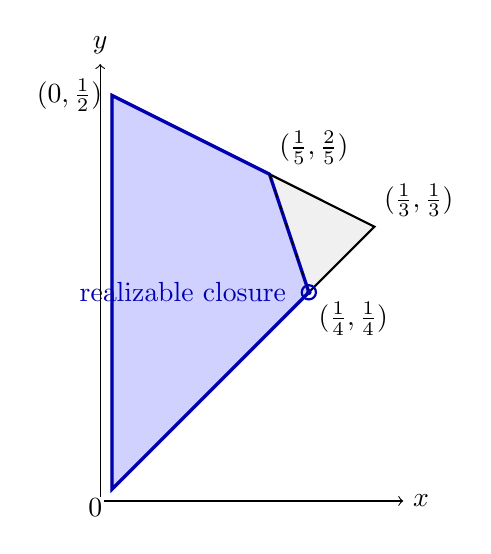
\begin{tikzpicture}[x=10cm,y=10cm]
  \fill[gray!12] (0,0)--(0,.5)--(.3333,.3333)--cycle;
  \fill[blue!18] (0,0)--(0,.5)--(.2,.4)--(.25,.25)--cycle;
  \draw[thick] (0,0)--(0,.5)--(.3333,.3333)--cycle;
  \draw[blue!70!black,very thick]
    (0,0)--(0,.5)--(.2,.4)--(.25,.25)--cycle;
  \draw[dashed] (.2,.4)--(.25,.25);
  \fill[blue!70!black] (.25,.25) circle (0.0035);
  \draw[blue!70!black,thick] (.25,.25) circle (0.009);
  \node[below left] at (0,0) {$0$};
  \node[left] at (0,.5) {$(0,\frac12)$};
  \node[above right] at (.2,.4) {$(\frac15,\frac25)$};
  \node[below right] at (.25,.25) {$(\frac14,\frac14)$};
  \node[above right] at (.3333,.3333) {$(\frac13,\frac13)$};
  \node[blue!70!black] at (.09,.25) {realizable closure};
  \draw[->] (-.01,-.015)--(.37,-.015) node[right] {$x$};
  \draw[->] (-.015,-.01)--(-.015,.54) node[above] {$y$};
\end{tikzpicture}
\caption{The trace-one ordered chamber (gray) and the closed spectral region
of $K_4-e$ (blue).  The dashed line is $z=2x$; at
$(1/4,1/4)$ the filled center records membership in the closure, while the
surrounding ring marks the strictly unattained ray $(x,x,2x)$.}
\label{fig:k4-region}
\end{figure}

\begin{corollary}[Exact spectral volume]\label{cor:k4-volume}
The normalized spectral volume of $K_4-e$ is
\[
  P(K_4-e)=\frac9{10}.
\]
\end{corollary}

\begin{proof}
The uniform measure on $\Delta_3$ is the distribution of
$(E_1,E_2,E_3)/(E_1+E_2+E_3)$ for independent unit exponentials.  Since the
condition is homogeneous, the excluded portion is
\[
  \Pr\bigl(E_{(3)}<2E_{(1)}\bigr).
\]
For a specified variable to be the minimum at $t$, the other two variables
must lie in $[t,2t]$.  Hence, up to a null boundary,
\[
  \Pr\bigl(E_{(3)}<2E_{(1)}\bigr)
  =3\int_0^\infty e^{-t}(e^{-t}-e^{-2t})^2\,dt
  =\frac1{10}.
\]
The complement has volume $9/10$.
\end{proof}

\begin{remark}[A genus-three multiscale boundary chart]
\label{rem:k4-multiscale}
A maximally pinched closed genus-three surface decomposes into four pairs of
pants, and one possible trivalent dual graph is $K_4$; cf.~\cite{EJT2026}.
In a two-scale degeneration for which five effective cuff conductances are
of order $s$ and the sixth is $o(s)$, the order-$s$ Burger graph Laplacian
has positive support $K_4-e$.  Thus $K_4-e$ occurs as a possible tangent
support on the boundary of the $K_4$ weight simplex.  This is only a
tangent-graph observation.  No exact hyperbolic spectral prescription or
maximal-cusp obstruction is asserted or used here.
\end{remark}

\section{Strict-support spectral-pair constructions}
\label{sec:strict-constructions}

We now prove Theorem~\ref{thm:spectral-pair-insertion-intro}.  The
construction is explicit except for one use of complete-graph flexibility.

\begin{proof}[Proof of Theorem~\ref{thm:spectral-pair-insertion-intro}]
Label the missing edge $12$, put $s=n-2$ and $\rho=n/s$, and let
$\Lambda'$ be the multiset left after deleting the two distinguished
occurrences $\alpha,\beta$ from $\Lambda$.
Define
\begin{equation}\label{eq:a-b-def}
  p=\frac{e_1-e_2}{\sqrt2},
  \qquad
  q=\sqrt{\frac{s}{2n}}(e_1+e_2)
  -\sqrt{\frac{2}{ns}}\sum_{j=3}^ne_j,
\end{equation}
and
\[
  W=\left\{v\in\R^n:v_1=v_2=0,\ \sum_{j=3}^nv_j=0\right\}.
\]
Then $p,q$ are orthonormal vectors in $\one^\perp$, and
\[
  \one^\perp=\operatorname{span}\{p,q\}\mathbin\perp W.
\]

Set
\begin{equation}\label{eq:u-v-eta}
  u=\frac{\alpha+\beta}{1+\rho},\qquad
  v=\rho u,\qquad
  \eta=\sqrt{(u-\alpha)(\beta-u)}.
\end{equation}
The assumption $\beta\ge\rho\alpha$ is equivalent to $u\ge\alpha$, while
$u\le\beta$ is automatic.  Thus $\eta$ is real.  Moreover,
\[
  u+v=\alpha+\beta,
  \qquad uv-\eta^2=\alpha\beta,
\]
so
\[
  M=\begin{pmatrix}u&\eta\\\eta&v\end{pmatrix}
\]
has eigenvalues $\alpha,\beta$.

Put
\begin{equation}\label{eq:delta}
  \delta=\frac{2v}{n}=\frac{\alpha+\beta}{n-1}.
\end{equation}
Every $t\in\Lambda'$ satisfies $t-\delta>0$.  By complete-graph flexibility
\cite[Theorem~2.5]{FGL2025}, there is a strictly weighted Laplacian
$R\in\SL(K_s)$ whose nonzero spectral multiset is
\begin{equation}\label{eq:R-spectrum}
  \{t-\delta:t\in\Lambda'\}.
\end{equation}
When $n=3$, the space $W$ is zero-dimensional and $\Lambda'$ is empty; take
$R=0$.  Let
\[
  H_s=I_s-\frac1sJ_s
\]
and embed $\delta H_s+R$ in the coordinates $3,\ldots,n$.  Define
\begin{equation}\label{eq:general-L}
  L=u pp^{\mathsf T}+\eta(pq^{\mathsf T}+qp^{\mathsf T})
    +vqq^{\mathsf T}+\iota(\delta H_s+R),
\end{equation}
where $\iota$ denotes the central-coordinate embedding.

The summands in \eqref{eq:general-L} preserve
\[
  \R^n=\operatorname{span}\{\one\}\mathbin\perp
  \operatorname{span}\{p,q\}\mathbin\perp W.
\]
The restriction to $\operatorname{span}\{p,q\}$ is $M$, and the restriction
to $W$ is $\delta I+R|_W$.  Equations \eqref{eq:R-spectrum} and
\eqref{eq:u-v-eta} therefore give
\[
  \Spec(L)=\{0\}\cup\Lambda.
\]

It remains to verify the graph pattern.  Since $v=nu/s$,
\[
  L_{12}=-\frac u2+\frac{vs}{2n}=0.
\]
For $j\ge3$, direct use of \eqref{eq:a-b-def} gives
\begin{equation}\label{eq:spoke-signs}
  L_{1j}=-\frac vn-\frac{\eta}{\sqrt{ns}}<0,
  \qquad
  L_{2j}=-\frac vn+\frac{\eta}{\sqrt{ns}}.
\end{equation}
Furthermore,
\[
  \eta^2=uv-\alpha\beta<uv=\frac{s}{n}v^2,
\]
so $\eta/\sqrt{ns}<v/n$ and the second entry in
\eqref{eq:spoke-signs} is also strictly negative.

Finally, for $3\le j\ne k\le n$, the $vqq^{\mathsf T}$ contribution is
$2v/(ns)$, whereas the $\delta H_s$ contribution is
$-\delta/s=-2v/(ns)$.  They cancel, leaving
\[
  L_{jk}=R_{jk}<0.
\]
Thus $L_{12}=0$, every other off-diagonal entry is strictly negative, and
$L\in\SL(K_n-e)$.
\end{proof}

\begin{corollary}[An ordered strict-support cone]\label{cor:ordered-cone}
Let $0<\lambda_2\le\cdots\le\lambda_n$.  If
\begin{equation}\label{eq:intro-cone}
  \lambda_3\ge\frac{n}{n-2}\lambda_2,
\end{equation}
then $\{0,\lambda_2,\ldots,\lambda_n\}$ has a strict $K_n-e$
realization.  The projective volume of this sufficient cone is
$(n-1)/(n+1)$.
\end{corollary}

\begin{proof}
Apply Theorem~\ref{thm:spectral-pair-insertion-intro} with
$(\alpha,\beta)=(\lambda_2,\lambda_3)$.  Every remaining eigenvalue is at
least $\beta$, while $(\alpha+\beta)/(n-1)<\beta$ for $n\ge4$; the case
$n=3$ has no remaining occurrence.  For the volume, use independent unit
exponentials.  If $T=E_{(1)}$ and $D=E_{(2)}-E_{(1)}$, then $T$ and $D$ are
independent exponentials of rates $n-1$ and $n-2$, respectively.  Hence
\[
  \Pr\left(E_{(2)}\ge\frac{n}{n-2}E_{(1)}\right)
  =\mathbb E(e^{-2T})=\frac{n-1}{n+1}.
\]
\end{proof}

At equality $\beta=\rho_n\alpha$, the insertion construction has $\eta=0$
and lands on the weak block locus, but all allowed edge weights remain
positive.  Equality in the condition $t>\delta$ is not included: in this
construction it would give $R$ an additional zero eigenvalue.

\begin{proof}[Proof of Theorem~\ref{thm:intro-one-spike}]
Necessity follows from Theorem~\ref{thm:missing-edge}.  For $n=3$, the
spectral-pair insertion theorem has no remaining occurrence and gives a
strict realization exactly when $b\ge3a$.  For $n=4$, the assertion is
Theorem~\ref{thm:k4-exact-intro} applied to $(a,a,b)$.

Suppose now that $n\ge5$, put $r=b/a$, and assume
$r\ge\rho_n$.  If $r<n-2$, choose $(\alpha,\beta)=(a,b)$ in
Theorem~\ref{thm:spectral-pair-insertion-intro}.  Every remaining occurrence
is $t=a$, and
\[
  a>\frac{a+b}{n-1}\iff r<n-2,
\]
so the resulting support is strict.

It remains to treat $r\ge n-2$.  Put
\[
  c=\frac{a}{n(b-a)}=\frac1{n(r-1)},
  \qquad
  h=\sqrt{\frac{1+2c}{2}}.
\]
Since $n\ge5$ and $r\ge n-2$, one has $0<c<1/6$.  Let $x,y$ be the two
positive roots of
\[
  z^2-hz+c=0
\]
and set
\[
  q=(x,y,-h,0,\ldots,0)^{\mathsf T}.
\]
The discriminant is $(1-6c)/2>0$, and
\[
  q^{\mathsf T}\one=x+y-h=0,
  \qquad
  \|q\|^2=x^2+y^2+h^2=2h^2-2c=1,
  \qquad q_1q_2=c.
\]
Every other product $q_iq_j$ is either negative or zero, and hence is
strictly smaller than $c$.  Therefore
\[
  L=aH_n+(b-a)qq^{\mathsf T}
\]
has spectrum $\{0,a^{(n-2)},b\}$ and satisfies
\[
  L_{12}=-\frac an+(b-a)c=0,
  \qquad
  L_{ij}=-\frac an+(b-a)q_iq_j<0
  \quad(\{i,j\}\ne\{1,2\}).
\]
Thus $L\in\SL(K_n-e)$, completing the classification.
\end{proof}

\section{Two disjoint missing edges: orbitopes and an exact rank-two slice}
\label{sec:m2-frontier}

The first higher-defect case already separates linear spectral obstructions
from the nonlinear support-incidence problem.  We begin with the general
linear family.  Write $H_n=I_n-J_n/n$ as in
Section~\ref{sec:prelim}.

\begin{theorem}[Complement-orbitope inequalities]
\label{thm:complement-orbitope}
Let $G$ be a graph on $n$ vertices, put $F=\overline G$, and let $W$ be any
symmetric zero-diagonal matrix supported on $E(F)$.  Write
\[
  \theta_1(W)\le\cdots\le\theta_{n-1}(W)
\]
for the eigenvalues of $H_nWH_n$ on $\one^\perp$.  If the ordered list
\[
  0=\lambda_1\le\lambda_2\le\cdots\le\lambda_n
\]
is realized by a relaxed weighted Laplacian on $G$, then
\begin{equation}\label{eq:complement-orbitope}
  \sum_{i=1}^{n-1}\lambda_{i+1}\theta_i(W)\ge0.
\end{equation}
\end{theorem}

\begin{proof}
The claim is immediate for the zero spectrum.  Otherwise put
\[
  B=I-\frac1{\lambda_n}L=\frac1nJ_n+C.
\]
On $\one^\perp$ the eigenvalues of $C$ in decreasing order are
$1-\lambda_i/\lambda_n$, $2\le i\le n$.  For every nonedge $ij$ one has
$C_{ij}=-1/n$.  Since $W$ is supported on the nonedges,
\[
  \tr(CW)=-\frac2n\sum_{ij\in E(F)}W_{ij}
  =\tr(H_nWH_n).
\]
Moreover $C=H_nCH_n$, and hence
\[
  \tr(CW)=\tr\bigl(C(H_nWH_n)\bigr).
\]
The von Neumann trace inequality on $\one^\perp$
\cite[Chapters~II--III]{Bhatia1997}, pairing the decreasing
eigenvalues of $C$ with the increasing $\theta_i(W)$, gives
\[
  \tr(CW)\ge
  \sum_{i=1}^{n-1}\left(1-\frac{\lambda_{i+1}}{\lambda_n}\right)
  \theta_i(W).
\]
The left side equals $\sum_i\theta_i(W)$.  Cancelling the trace terms and
multiplying by $\lambda_n$ proves \eqref{eq:complement-orbitope}.
\end{proof}

Now take $F=M_2$ with missing edges $12$ and $34$, and put
\begin{equation}\label{eq:m2-h}
  h=\frac{n-4}{n}.
\end{equation}
The symmetric choice in Theorem~\ref{thm:complement-orbitope} gives the
facet
\begin{equation}\label{eq:m2-facet}
  \lambda_n+h\lambda_{n-1}\ge\lambda_2+\lambda_3.
\end{equation}
Allowing arbitrary real coefficients on the two missing edges produces no
additional linear information.

\begin{theorem}[Collapse of the $M_2$ complement orbitope]
\label{thm:m2-orbitope-collapse}
Let $n\ge5$.  For $x,y\in\R$, let $W(x,y)$ be the symmetric zero-diagonal
matrix whose only possibly nonzero upper-triangular entries are
$W_{12}=x$ and $W_{34}=y$.  Every nonnegative ordered list satisfying
\eqref{eq:m2-facet} also satisfies
\[
  \sum_{i=1}^{n-1}\lambda_{i+1}\theta_i(W(x,y))\ge0
  \qquad(x,y\in\R).
\]
Conversely, the inequality for $x=y=1$ is exactly
\eqref{eq:m2-facet}.  Thus, in the ordered chamber, the complete family of
complement-orbitope inequalities supported on $M_2$ is equivalent to the
single symmetric facet \eqref{eq:m2-facet}.
\end{theorem}

\begin{proof}
Put $m=n-1$, $\ell=(\lambda_2,\ldots,\lambda_n)$, and
\[
  v_j=(0^{j-1},1^{m-j+1})\qquad(1\le j\le m).
\]
Every nonnegative ordered list has a unique expansion
$\ell=\sum_{j=1}^m d_jv_j$ with $d_j\ge0$.  Define
\[
  \mathcal F(\ell)=\ell_1+\ell_2-h\ell_{m-1}-\ell_m.
\]
Then \eqref{eq:m2-facet} is $\mathcal F(\ell)\le0$, and
\[
 \mathcal F(v_1)=1-h,\qquad \mathcal F(v_2)=-h,
\]
\[
 \mathcal F(v_j)=-(1+h)\quad(3\le j\le m-1),
 \qquad \mathcal F(v_m)=-1.
\]
There is exactly one positive coefficient.  In the $d$-coordinates, the
extreme rays of $d_j\ge0$, $\mathcal F(\ell)\le0$ are therefore
\[
 v_j\quad(2\le j\le m),
 \qquad
 -\mathcal F(v_j)v_1+(1-h)v_j\quad(2\le j\le m).
\]

Let $\theta_1\le\cdots\le\theta_m$ be the spectrum of
$H_nW(x,y)H_n$ on $\one^\perp$, and put
$T_j=\sum_{i=j}^m\theta_i$.  Testing $\theta\cdot\ell\ge0$ on the displayed
extreme rays reduces the assertion to
\begin{align}
 T_j&\ge0 &&(2\le j\le m),\label{eq:m2-tail-1}\\
 hT_1+(1-h)T_2&\ge0,\label{eq:m2-tail-2}\\
 (1+h)T_1+(1-h)T_j&\ge0 &&(3\le j\le m-1),
 \label{eq:m2-tail-3}\\
 T_1+(1-h)T_m&\ge0.\label{eq:m2-tail-4}
\end{align}
The edge-difference vectors $e_1-e_2$ and $e_3-e_4$ are eigenvectors of
the compression with eigenvalues $-x$ and $-y$.  The subspace supported on
vertices $5,\ldots,n$ with coordinate sum zero contributes $0^{n-5}$.
On the remaining two-dimensional invariant quotient, a direct compression
in the two pair-sum directions has trace $(n-2)(x+y)/n$ and determinant
$(n-4)xy/n$.  Hence the characteristic polynomial is
\begin{equation}\label{eq:m2-compression-charpoly}
 z^{n-5}(z+x)(z+y)
 \left(z^2-\frac{(n-2)(x+y)}n z+\frac{(n-4)xy}{n}\right).
\end{equation}

Suppose first that $x\ge y\ge0$.  If $r_-\le r_+$ are the two quadratic
roots in \eqref{eq:m2-compression-charpoly}, the ordered spectrum is
\[
 -x,-y,0^{n-5},r_-,r_+.
\]
Consequently
\[
 T_1=-\frac{2(x+y)}n,\qquad
 T_2=x-\frac{2(x+y)}n,\qquad
 T_j=\frac{n-2}{n}(x+y)\quad(3\le j\le m-1).
\]
These quantities give \eqref{eq:m2-tail-1}; the left sides of
\eqref{eq:m2-tail-2} and \eqref{eq:m2-tail-3} reduce respectively to
$2(x-y)/n$ and $0$.  Evaluating the quadratic factor at $(x+y)/2$ gives
\[
 \frac{n-4}{n}\left(xy-\frac{(x+y)^2}{4}\right)\le0,
\]
so $r_+\ge(x+y)/2$ and \eqref{eq:m2-tail-4} follows.  If $x,y\le0$,
negating the preceding spectrum shows directly that $T_1$ and all the
tails occurring in \eqref{eq:m2-tail-1}--\eqref{eq:m2-tail-4} are
nonnegative.

It remains to take $x=a>0$ and $y=-b<0$.  Write the two quadratic roots as
$-u<0<v$.  They satisfy
\begin{equation}\label{eq:m2-mixed-roots}
 v-u=\frac{n-2}{n}(a-b),\qquad uv=\frac{n-4}{n}ab.
\end{equation}
The negative eigenvalues are $-a,-u$, the positive eigenvalues are $b,v$,
and all remaining eigenvalues are zero.  Put
$A=\max(a,u)$ and $B=\max(b,v)$.  Then
\[
 T_1=\frac{2(b-a)}n,\qquad T_2=T_1+A,
\]
while every tail in \eqref{eq:m2-tail-3} is $b+v$.  This proves
\eqref{eq:m2-tail-1}.  The left side of \eqref{eq:m2-tail-2} is
\[
 \frac{2(b-a)+4A}{n}>0.
\]
If $b\ge a$, \eqref{eq:m2-tail-3} and \eqref{eq:m2-tail-4} are immediate.
If $a>b$, multiplying the left side of \eqref{eq:m2-tail-3} by $n/4$ and
using \eqref{eq:m2-mixed-roots} gives
\[
 b+v-\frac{n-2}{n}(a-b)=b+u>0.
\]
Also
$B\ge v\ge(n-2)(a-b)/n>(a-b)/2$, which proves
\eqref{eq:m2-tail-4}.  Swapping $x$ and $y$ leaves the spectrum unchanged,
so all real cases have been covered.

For $x=y=1$, \eqref{eq:m2-compression-charpoly} gives
\[
 -1,-1,0^{n-5},h,1,
\]
and the orbitope inequality is precisely \eqref{eq:m2-facet}.
\end{proof}

The collapse theorem is a limitation theorem: varying a linear witness on
the two missing edges cannot prove more than \eqref{eq:m2-facet}.  The full
$K_n-M_2$ cone still requires a nonlinear fixed-spectrum orbit-incidence
argument.  The following slice can nevertheless be closed exactly.

\begin{theorem}[Exact two-level top-rank-two slice]
\label{thm:m2-ranktwo-slice}
Let $n\ge6$ and $0<a<b$.  Put $g=b/a-1$.  The spectrum
\begin{equation}\label{eq:m2-ranktwo-spectrum}
 \{0,a^{(n-3)},b^{(2)}\}
\end{equation}
has a relaxed $K_n-M_2$ realization if and only if
\[
 g\ge\frac2{n-2}.
\]
It has a strict $K_n-M_2$ realization if and only if
\[
 \begin{cases}
  g\ge 2/(n-2),&n\ge7,\\
  g>1/2,&n=6.
 \end{cases}
\]
Thus the unique boundary exception in this range occurs for $n=6$ and
$b/a=3/2$.
\end{theorem}

\begin{proof}
Put
\[
 c=\frac1{ng}.
\]
A rank-two orthogonal projection $P$ with $P\one=0$ gives
\[
 L=aH_n+agP.
\]
This matrix has spectrum \eqref{eq:m2-ranktwo-spectrum}, and, for $i\ne j$,
\[
 L_{ij}=ag(P_{ij}-c).
\]
Hence it has exact strict $K_n-M_2$ support if and only if
\begin{equation}\label{eq:m2-projection-criterion}
 P_{12}=P_{34}=c,\qquad P_{ij}<c\quad(ij\ne12,34).
\end{equation}
For relaxed support, the final strict inequalities are replaced by
$P_{ij}\le c$.

Substitution in \eqref{eq:m2-facet} gives the necessary condition
$g\ge2/(n-2)$.  At $n=6$ and $g=1/2$ one has $c=1/3$.  If $A_F$ is the
adjacency matrix of the matching, then
\[
 \Spec(H_6A_FH_6|_{\one^\perp})=(-1,-1,0,1/3,1).
\]
For any rank-two projection satisfying the two contacts,
\[
 \tr(PH_6A_FH_6)=2(P_{12}+P_{34})=\frac43.
\]
This is the rank-two Ky Fan maximum $1+1/3$
\cite[Chapter~III]{Bhatia1997}.  Equality forces
$\operatorname{im}P$ to be the sum of the two positive eigenspaces and
therefore forces
\[
 P=P_0:=\frac16
 \begin{pmatrix}
 2&2&-1&-1&-1&-1\\
 2&2&-1&-1&-1&-1\\
 -1&-1&2&2&-1&-1\\
 -1&-1&2&2&-1&-1\\
 -1&-1&-1&-1&2&2\\
 -1&-1&-1&-1&2&2
 \end{pmatrix}.
\]
In particular $(P_0)_{56}=c$, so a third zero edge is forced and exact
strict support is impossible at this boundary point.  The same $P_0$ does
give a relaxed realization.

It remains to construct projections satisfying
\eqref{eq:m2-projection-criterion}.  Put $q=n-4$ and define
\[
 A=\frac12(1,1,-1,-1,0^q),\qquad
 B=(u,u,u,u,v,\ldots,v),
\]
where
\[
 u=\sqrt{\frac q{4n}},\qquad v=-\frac2{\sqrt{nq}}.
\]
Also set
\[
 E=\frac1{\sqrt2}(0,0,0,0,1,-1,0^{q-2}).
\]
These vectors lie in $\one^\perp$ and $A,B,E$ are mutually orthonormal.
For $0\le s\le\pi/2$ let
\[
 B_s=(\cos s)B+(\sin s)E,\qquad
 P_s=AA^{\mathsf T}+B_sB_s^{\mathsf T}.
\]
Then
\begin{equation}\label{eq:m2-contact-large-c}
 (P_s)_{12}=(P_s)_{34}
 =\frac14+\frac q{4n}\cos^2s,
\end{equation}
so this family covers
$1/4\le c\le(n-2)/(2n)$.

For completeness, we verify strictness.  Cross-pair entries among the first
four vertices equal $c-1/2$.  Every endpoint--core entry is at most
$u/(2\sqrt2)<1/4\le c$.  The only potentially largest core--core entry is
\[
 v^2\cos^2s+\frac{|v|}{\sqrt2}\cos s\sin s.
\]
Writing $d=u^2-v^2$, its difference from $c$ has minimum
\[
 \frac14+\frac d2-\frac12\sqrt{d^2+\frac{v^2}{2}}.
\]
Here $1/2+d=(3q-4)/(4q)>0$ for $q\ge2$, so squaring introduces no change
of sign.  Positivity is equivalent to
\[
 \frac14+u^2-\frac32v^2>0,
\]
or, after multiplication by $4q(q+4)$,
$2(q+6)(q-2)>0$.  Hence every other entry is strictly below $c$ for
$n\ge7$, including at $s=0$.  For $n=6$ the same conclusion holds for
$s>0$, while
\[
 c-(P_s)_{56}=\frac34\sin^2s;
\]
the sole failure is $s=0$.  Thus \eqref{eq:m2-contact-large-c} covers the
required range down to $c=1/4$.

For $0<c\le1/4$, define
\[
 C=\frac12(1,-1,1,-1,0^{n-4})
\]
and, for $0\le t<\pi/4$, put
\[
 A_t=(\cos t)A+(\sin t)C,\qquad
 Q_t=A_tA_t^{\mathsf T}+EE^{\mathsf T}.
\]
Then
\[
 (Q_t)_{12}=(Q_t)_{34}=\frac{\cos2t}{4}.
\]
The other entries among the first four vertices are
\[
 -c,\quad-\frac{(\cos t+\sin t)^2}{4},\quad
 -\frac{(\cos t-\sin t)^2}{4},\quad-c;
\]
all endpoint--core entries are zero, $(Q_t)_{56}=-1/2$, and every remaining
core entry is zero.  They are all strictly below $c$.

The two constructions therefore prove sufficiency for $n\ge7$ when
$c\le(n-2)/(2n)$, equivalently $g\ge2/(n-2)$, and for $n=6$ when
$c<1/3$, equivalently $g>1/2$.  Necessity and the order-six exception were
proved above; $P_0$ supplies the missing relaxed order-six endpoint.
\end{proof}

\begin{remark}[Scope of the slice]
Theorem~\ref{thm:m2-ranktwo-slice} does not treat $n=5$, other intermediate
eigenspace ranks, or arbitrary spectra, and it does not assert that
\eqref{eq:m2-facet} is sufficient for the full $K_n-M_2$ cone.  The
repeated-top slice of rank $n-2$ has a separate exact-support obstruction.
\end{remark}

\section{Exact spectral volume and the last-edge gap}\label{sec:volume}

The half-space description in Theorem~\ref{thm:exact-kne-cone} makes the
spectral volume exactly computable.

\begin{theorem}[Exact spectral volume of $K_n-e$]
\label{thm:volume-bound}
For every $n\ge3$,
\begin{equation}\label{eq:volume-bound}
  P(K_n-e)
  =1-\binom{(n-2)(n+1)/2}{n-2}^{-1}.
\end{equation}
Consequently $P(K_n-e)\to1$.
\end{theorem}

\begin{proof}
Put $m=n-1$.  A uniformly distributed point of $\Delta_m$ is represented by
\[
  \left(\frac{E_1}{\sum_iE_i},\ldots,
  \frac{E_m}{\sum_iE_i}\right),
\]
where $E_1,\ldots,E_m$ are independent unit exponentials.  We use the
classical exponential representation and order-statistic spacings
\cite{Renyi1953}.  By Theorem~\ref{thm:exact-kne-cone}, the excluded event is
\[
  E_{(m)}<\left(1+\frac{2}{m-1}\right)E_{(1)}.
\]
With $c=2/(m-1)$, conditioning on which variable is minimal and on its value
gives
\begin{align*}
  \Pr(E_{(m)}<(1+c)E_{(1)})
  &=m\int_0^\infty e^{-mt}(1-e^{-ct})^{m-1}\,dt\\
  &=\frac{m}{c}B\left(\frac{m}{c},m\right)\\
  &=\binom{(n-2)(n+1)/2}{n-2}^{-1}.
\end{align*}
Here $m/c=m(m-1)/2$ and
$m/c+m-1=(n-2)(n+1)/2$.  
Taking the complement proves the formula.
\end{proof}

\begin{corollary}[The exact last-edge gap]\label{cor:last-edge}
For every $n\ge3$,
\begin{equation}\label{eq:exact-last-edge}
  P(K_n)-P(K_n-e)
  =\binom{(n-2)(n+1)/2}{n-2}^{-1}.
\end{equation}
Writing $k=n-2$ and $N=k(k+3)/2$, one has
\begin{equation}\label{eq:last-edge-full-asymptotic}
  1-P(K_n-e)
  \sim e^{-2}\sqrt{2\pi k}
  \left(\frac{2}{ek}\right)^k.
\end{equation}
Moreover,
\[
  P(K_{n+1}-e)>P(K_n-e),
\]
so one-step suspension monotonicity holds on the entire one-missing-edge
family.
\end{corollary}

\begin{proof}
The complete-graph theorem gives $P(K_n)=1$, proving
\eqref{eq:exact-last-edge}.  Write
\[
  N^{\underline{k}}=N(N-1)\cdots(N-k+1).
\]
Then
\[
  1-P(K_n-e)=\frac{k!}{N^{\underline{k}}},
  \qquad
  \frac{N^{\underline{k}}}{N^k}
  =\prod_{j=0}^{k-1}\left(1-\frac jN\right)\longrightarrow e^{-1}.
\]
Together with Stirling's formula and
$N^k\sim e^3(k^2/2)^k$, this gives
\eqref{eq:last-edge-full-asymptotic}.

Finally, the binomial coefficient in \eqref{eq:exact-last-edge} increases
strictly with $n$.  Indeed,
\[
  \binom{N+k+2}{k+1}
  \ge\binom{N+1}{k+1}
  =\frac{N+1}{k+1}\binom Nk
  >\binom Nk.
\]
Thus its reciprocal decreases strictly.
\end{proof}

\begin{remark}
This does not decide whether there is a positive edge-gain lower bound
uniform over all connected noncomplete graphs of a fixed order $n$.  It does
show that any such constant satisfies
\[
  c_n\le\binom{(n-2)(n+1)/2}{n-2}^{-1}.
\]
If disconnected graphs are admitted literally, zero-gap examples already
make an unrestricted version degenerate.
\end{remark}

\section{Fixed-core joins and iterated suspension}\label{sec:fixed-core}

For graphs on disjoint vertex sets, write $G\vee H$ for their join: all
edges of $G$ and $H$ are retained and every vertex of $G$ is joined to every
vertex of $H$.  Thus the $k$-fold suspension of $G$ is $G\vee K_k$.  The
one-vertex suspension formula goes back at least to Colin de Verdi\`ere
\cite{CdV1988}; related Laplacian formulas for generalized graph
compositions appear in \cite{Gerbaud2010}, and the block formula below is the
weighted join construction of \cite[Lemma~2.4]{FGL2025}.  We do not claim the
join identity itself as new; the new step is its probabilistic use to control
spectral volume.

We first record the local input that allows a fixed graph to absorb a
prescribed finite portion of a large spectrum.

\begin{lemma}[A spectral box]\label{lem:spectral-box}
Let $H$ be a connected graph on $m\ge2$ vertices.  There are bounded open
intervals
\[
  I_1<I_2<\cdots<I_{m-1}\subset\R_{>0}
\]
such that every tuple
\[
  (\mu_1,\ldots,\mu_{m-1})\in I_1\times\cdots\times I_{m-1}
\]
is the nonzero spectrum of some matrix in $\SL(H)$.
\end{lemma}

\begin{proof}
By \cite[Theorem~3.11]{CFGL2026}, the class $\SL(H)$ contains a matrix
$A$ with the SSPWL.  Choose a real symmetric matrix $M$ with
$M\one_m=0$ and simple spectrum, arbitrarily close to $A$.  The
Bifurcation lemma \cite[Lemma~2.12]{CFGL2026} gives
$A_0\in\SL(H)$ with $\Spec(A_0)=\Spec(M)$ and the SSPWL.  Thus
\[
  \Spec(A_0)=\{0,\mu_1^*,\ldots,\mu_{m-1}^*\},
  \qquad 0<\mu_1^*<\cdots<\mu_{m-1}^*.
\]

Choose an orthonormal eigenbasis of $A_0$ whose first vector is
$m^{-1/2}\one_m$.  Replacing the nonzero diagonal entries in this basis by
any sufficiently close tuple $(\mu_1,\ldots,\mu_{m-1})$ produces a matrix
$M'$ with $M'\one_m=0$ arbitrarily close to $A_0$.
Another application of the Bifurcation lemma gives a matrix in $\SL(H)$
with spectrum $\Spec(M')$.  Taking sufficiently small pairwise disjoint
intervals around the $\mu_i^*$ proves the claim.  This is also the local
spectral openness encoded by the full-rank Jacobian criterion in
\cite[Theorem~3.8]{CFGL2026}.
\end{proof}

\begin{lemma}[Join spectrum]\label{lem:join-spectrum}
Let $H$ have $m$ vertices, let $k\ge1$, and put $N=m+k$.  Suppose
\[
  \Spec(A)=\{0,\mu_1,\ldots,\mu_{m-1}\},
  \qquad A\in\SL(H),
\]
and
\[
  \Spec(B)=\{0,\nu_1,\ldots,\nu_{k-1}\},
  \qquad B\in\SL(K_k),
\]
where for $k=1$ the second list is empty and $B=(0)$.  For $c>0$, set
\begin{equation}\label{eq:join-matrix}
  L(A,B,c)=
  \begin{pmatrix}
    A+kcI_m&-cJ_{m,k}\\
    -cJ_{k,m}&B+mcI_k
  \end{pmatrix}.
\end{equation}
Then $L(A,B,c)\in\SL(H\vee K_k)$ and
\begin{equation}\label{eq:join-spectrum}
  \Spec L(A,B,c)
  =
  \{0,Nc\}
  \cup\{\mu_i+kc:1\le i\le m-1\}
  \cup\{\nu_j+mc:1\le j\le k-1\}.
\end{equation}
\end{lemma}

\begin{proof}
The matrix in \eqref{eq:join-matrix} retains the weights of $A$ and $B$ and
assigns weight $c$ to every joining edge.  The four mutually orthogonal
spaces
\[
  \operatorname{span}\{\one_N\},\quad
  \{(u,0):u\perp\one_m\},\quad
  \{(0,v):v\perp\one_k\},\quad
  \operatorname{span}\{(k\one_m,-m\one_k)\}
\]
are invariant.  The corresponding eigenvalues are, respectively,
$0$, the numbers $\mu_i+kc$, the numbers $\nu_j+mc$, and $Nc$, proving
\eqref{eq:join-spectrum}.
\end{proof}

We now combine this deterministic splitting with exponential order
statistics.  The quantitative estimate will also verify that all edge
weights may be kept strictly positive.

\begin{theorem}[Fixed-core join theorem]\label{thm:fixed-core}
Let $H$ be a fixed connected graph on $m\ge2$ vertices.  There are constants
$\eta>0$ and $p_1,\ldots,p_{m-1}\in(0,1)$, depending only on $H$, such that
for every $k\ge1$, with $N=m+k$,
\begin{equation}\label{eq:fixed-core-explicit}
  P(H\vee K_k)
  \ge
  1-
  \exp\left(-\frac{\eta N(N-1)}{m}\right)
  -
  \sum_{i=1}^{m-1}(1-p_i)^{N-2}.
\end{equation}
In particular, there are $C_H,c_H>0$ such that
\begin{equation}\label{eq:fixed-core-rate}
  1-P(H\vee K_k)\le C_He^{-c_Hk}.
\end{equation}
Every spectrum counted in the lower bound has a realization with strictly
positive weight on every edge of $H\vee K_k$.
\end{theorem}

\begin{proof}
Choose the spectral box $I_1\times\cdots\times I_{m-1}$ from
Lemma~\ref{lem:spectral-box}.  Choose nonempty open intervals
$J_i\Subset I_i$ and $\eta>0$ such that
\begin{equation}\label{eq:shifted-box}
  J_i+[0,\eta]\subset I_i
  \qquad(1\le i\le m-1).
\end{equation}
For a unit exponential random variable $Y$, put
\[
  p_i=\Pr(Y\in J_i)>0.
\]

Let $X_1,\ldots,X_{N-1}$ be independent unit exponential random variables.
Their normalization by $\sum_jX_j$ is uniformly distributed on the
trace-one simplex.  Since spectral realizability is homogeneous, it suffices
to realize the unnormalized multiset $\{X_1,\ldots,X_{N-1}\}$.

Let $T=\min_jX_j$.  Almost surely the minimum is unique.  Conditional on
its minimizing index, the exponential memoryless property says that the
$N-2$ residual differences
\[
  Y_\ell=X_\ell-T
\]
are independent unit exponentials, independent of $T$, while $T$ is
exponential with rate $N-1$.  Consider the event
\begin{equation}\label{eq:capture-event}
  \mathcal A=
  \left\{\frac{mT}{N}\le\eta\right\}
  \cap
  \bigcap_{i=1}^{m-1}
  \left\{\text{some $Y_\ell$ belongs to $J_i$}\right\}.
\end{equation}
The intervals $J_i$ are disjoint, so on $\mathcal A$ the selected indices
may be chosen distinctly.  A union bound gives
\begin{align}
  \Pr(\mathcal A^c)
  &\le
  \Pr\left(T>\frac{\eta N}{m}\right)
  +
  \sum_{i=1}^{m-1}
  \Pr\left(Y_\ell\notin J_i\text{ for every }\ell\right)\notag\\
  &=
  \exp\left(-\frac{\eta N(N-1)}m\right)
  +
  \sum_{i=1}^{m-1}(1-p_i)^{N-2}.
  \label{eq:capture-error}
\end{align}

Suppose $\mathcal A$ occurs and put
\[
  c=\frac{T}{N},
  \qquad
  \mu_i=Y_{\ell_i}+\frac{mT}{N},
\]
where $Y_{\ell_i}\in J_i$.  By \eqref{eq:shifted-box}, the tuple
$(\mu_1,\ldots,\mu_{m-1})$ lies in the spectral box, so it is realized by
some $A\in\SL(H)$.  For every unselected residual $Y_\ell$, set
\[
  \nu_\ell=T+Y_\ell-mc
  =Y_\ell+\frac{kT}{N}>0.
\]
There are exactly $k-1$ such numbers.  Complete-graph flexibility
\cite[Theorem~2.5]{FGL2025} provides $B\in\SL(K_k)$ having them as its
nonzero spectrum; for $k=1$ this list is empty and $B=(0)$.

Apply Lemma~\ref{lem:join-spectrum}.  Its distinguished eigenvalue is
$Nc=T$.  For each selected index,
\[
  \mu_i+kc
  =Y_{\ell_i}+\frac{mT}{N}+\frac{kT}{N}
  =T+Y_{\ell_i},
\]
and for every unselected index,
\[
  \nu_\ell+mc=T+Y_\ell.
\]
Thus $L(A,B,c)$ realizes the entire target multiset.  Since $A$ and $B$ have
strict support and $c=T/N>0$, the realization has strict support on
$H\vee K_k$.  Equation \eqref{eq:capture-error} proves
\eqref{eq:fixed-core-explicit}.  The right side is $O_H(e^{-c_Hk})$ for a
positive $c_H$, proving \eqref{eq:fixed-core-rate}.
\end{proof}

\begin{proof}[Proof of Theorem~\ref{thm:intro-suspension}]
Associativity of graph join gives $\susp^k(G)=G\vee K_k$.  If $G$ is
connected and has at least two vertices, the conclusion is
Theorem~\ref{thm:fixed-core}.  If $G$ is disconnected, then
$H=G\vee K_1$ is connected and, for $k\ge2$,
\[
  G\vee K_k=H\vee K_{k-1}.
\]
Apply Theorem~\ref{thm:fixed-core} to $H$ and absorb the index shift into the
constant; increasing that constant also covers the single value $k=1$.
If $G=K_1$, then $G\vee K_k=K_{k+1}$ and $P(G\vee K_k)=1$.
Thus \cite[Question~5]{EJT2026} has an affirmative answer, with exponential
convergence.
\end{proof}

\begin{theorem}[Uniform finite-defect flexibility]\label{thm:finite-defect}
For every integer $r\ge0$ there are constants $C_r,c_r>0$ such that, for
every $n\ge2$,
\begin{equation}\label{eq:finite-defect}
  \sup_{\substack{|V(G)|=n\\ |E(\overline G)|\le r}}
  \bigl(1-P(G)\bigr)
  \le C_re^{-c_rn}.
\end{equation}
Consequently,
\[
  \lim_{n\to\infty}
  \inf_{\substack{|V(G)|=n\\ |E(\overline G)|\le r}}P(G)=1.
\]
\end{theorem}

\begin{proof}
The case $r=0$ is the complete-graph theorem.  Suppose $r\ge1$ and first
take $n\ge2r+2$.  If $G=K_n$ there is nothing to prove.  Otherwise let $S$
be the set of endpoints of the edges of $\overline G$.  Then
$2\le |S|\le2r$.  Choose $u\in V(G)\setminus S$ and put
\[
  H=G[S\cup\{u\}].
\]
The vertex $u$ is adjacent to every vertex of $S$, so $H$ is connected.
Every vertex outside $S$ is universal in $G$, and hence
\[
  G=H\vee K_{n-|V(H)|},
  \qquad |V(H)|\le2r+1.
\]
For fixed $r$, only finitely many isomorphism types of such connected cores
$H$ occur.  Apply Theorem~\ref{thm:fixed-core} to each type and take the
minimum of their positive rates and the maximum of their constants.  This
gives \eqref{eq:finite-defect} for $n\ge2r+2$.  There are only finitely many
smaller orders, and increasing $C_r$ absorbs them because $0\le P(G)\le1$.
\end{proof}

\section{Tail-admissible cores and the optimal defect exponent}
\label{sec:tail-admissible}

The exponential estimate in Theorem~\ref{thm:fixed-core} uses one fixed
spectral box.  For several small cores the exact region contains a global
cone on which the largest eigenvalue is allowed to move.  Overlapping the
corresponding join charts improves the error to the optimal scale
$\exp\{-n\log n+O(n)\}$.

\begin{definition}[Tail-admissible core]\label{def:tail-admissible}
Let $H$ be a graph on $m\ge3$ vertices.  For
$1\le\ell\le m-2$ and $A>0$, put
\[
  \mathcal T_{A,\ell}^{(m)}=
  \left\{0<\mu_1\le\cdots\le\mu_{m-1}:
    \mu_{m-1}>A\sum_{i=1}^{\ell}\mu_i\right\}.
\]
We call $H$ \emph{relaxedly $(A,\ell)$-tail-admissible} if this cone is
contained in $\mathcal E_{\ge0}(H)$, and \emph{strictly
$(A,\ell)$-tail-admissible} if it is contained in
$\mathcal E_{>0}(H)$.  The middle coordinates are unrestricted apart from
ordering.  The argument below requires $A\ell>1$.
\end{definition}

We first isolate the probabilistic estimate used by the moving-anchor
construction.  Order statistics are denoted by parentheses; ties have
probability zero.

\begin{lemma}[Exponential clustering]\label{lem:exponential-clustering}
Let $T\sim\operatorname{Exp}(n-1)$ and let
$Y_1,\ldots,Y_d$ be independent unit exponentials, independent of $T$, where
$d=n-2$.  Suppose that for fixed constants $C,K>0$,
\[
  0\le d-r\le K\frac n{\log n},
  \qquad 0<\delta\le\frac Cn.
\]
Then
\begin{equation}\label{eq:clustering-bound}
  \Pr\left(Y_{(d)}-Y_{(d-r+1)}
    \le\delta\bigl(Y_{(d)}+T\bigr)\right)
  \le\exp\{-n\log n+O_{C,K}(n)\}.
\end{equation}
\end{lemma}

\begin{proof}
Condition on $T=t$, and write $a=\delta t$, $Z=Y_{(d)}$, and
$w(z)=\delta z+a$.  If $Z\le2a$, then
\[
  \Pr(Z\le2a\mid T=t)=(1-e^{-2a})^d\le(2a)^d.
\]
Averaging over $T$ bounds this contribution by
\begin{equation}\label{eq:small-maximum}
  (2\delta)^d\mathbb E(T^d)
  =(2\delta)^d\frac{d!}{(n-1)^d}
  \le\exp\{-n\log n+O_{C,K}(n)\}.
\end{equation}

For $z>2a$ and all sufficiently large $n$, one has $w(z)<z$.  The
exponential mass of $[z-w(z),z]$ is at most
\[
  p(z,a)=e^{-z+w(z)}-e^{-z}
  \le e^{-z}w(z)e^{w(z)}.
\]
Choose the coordinate attaining the maximum and the other $r-1$ coordinates
in the cluster.  Leaving the remaining coordinates unrestricted gives
\begin{align}
 &d\binom{d-1}{r-1}
   \int_{2a}^{\infty}e^{-z}p(z,a)^{r-1}\,dz \notag\\
 &\quad\le d\binom{d-1}{r-1}e^{(r-1)a}
 \int_0^\infty e^{-\beta z}(\delta z+a)^{r-1}\,dz,
 \label{eq:large-maximum-integral}
\end{align}
where $\beta=r-(r-1)\delta$.  The integral is at most
\begin{equation}\label{eq:cluster-gamma}
  2^{r-2}\left(
    \frac{\delta^{r-1}\Gamma(r)}{\beta^r}
    +\frac{a^{r-1}}\beta\right).
\end{equation}
Put $\lambda=n-1$.  Since $a=\delta T$,
\begin{align*}
  \mathbb E e^{(r-1)a}
    &=\frac\lambda{\lambda-(r-1)\delta},\\
  \mathbb E\!\left(e^{(r-1)a}a^{r-1}\right)
    &=\frac{\delta^{r-1}\lambda\Gamma(r)}
      {(\lambda-(r-1)\delta)^r}.
\end{align*}
Here $\beta\ge r/2$ and
$\lambda-(r-1)\delta\ge\lambda/2$ for large $n$.  Thus the average of
\eqref{eq:large-maximum-integral} is at most
\[
  \delta^{r-1}\exp\{O_{C,K}(n)\}
  \le\exp\{-n\log n+O_{C,K}(n)\},
\]
because $\log\binom{d-1}{r-1}=O_K(n)$,
$\Gamma(r)/(r/2)^r=\exp\{O(n)\}$, and
$r=n-O_K(n/\log n)$.  Combining this with
\eqref{eq:small-maximum} proves the lemma.
\end{proof}

\begin{theorem}[Moving-anchor join theorem]\label{thm:moving-anchor}
Let $H$ be a fixed connected noncomplete graph on $m\ge3$ vertices.  Suppose
that $H$ is relaxedly $(A,\ell)$-tail-admissible for some
$1\le\ell\le m-2$ with $A\ell>1$.  Then there are $C_H>0$ and $n_H$ such
that, for $n\ge n_H$,
\begin{equation}\label{eq:moving-anchor-two-sided}
  \binom{(n-2)(n+1)/2}{n-2}^{-1}
  \le1-P(H\vee K_{n-m})
  \le\exp\{-n\log n+C_Hn\}.
\end{equation}
In particular,
\begin{equation}\label{eq:tail-law}
  1-P(H\vee K_{n-m})=\exp\{-n\log n+O_H(n)\}.
\end{equation}
If $H$ is strictly $(A,\ell)$-tail-admissible, every spectrum in the construction is
realized with strict support.  Under relaxed tail-admissibility, the same
volume conclusion holds; the possible strict/relaxed discrepancy is null.
\end{theorem}

\begin{proof}
Set
\[
  M=\left\lfloor\frac n2\right\rfloor,
  \quad s=M-m,
  \quad k=n-M,
  \quad d=n-2,
  \quad J=\left\lfloor\frac n{\log n}\right\rfloor.
\]
For large $n$, $s\ge1$, and associativity gives
\begin{equation}\label{eq:nested-join}
  H\vee K_{n-m}=(H\vee K_s)\vee K_k.
\end{equation}

Let $X_1,\ldots,X_{n-1}$ be independent unit exponentials and let
$T=\min_iX_i$.  After deleting the minimizing coordinate, memorylessness
gives $d$ independent unit-exponential residuals, independent of $T$; write
their order statistics as $0<y_1<\cdots<y_d$.  Moreover,
$T\sim\operatorname{Exp}(n-1)$.

For the outer join in \eqref{eq:nested-join}, take cross weight $c_0=T/n$.
A residual $y_i$ assigned to the $M$-vertex core must be realized there as
\[
  a_i=y_i+\frac{MT}{n}.
\]
Every unselected residual is assigned to $K_k$ as the positive eigenvalue
$y_i+kT/n$.  It remains to realize $M-1$ of the $a_i$ on $H\vee K_s$.

Fix an anchor $1\le j\le J$ and put
\[
  c_1=\frac{a_j}{M},\qquad
  b_j=mc_1=\frac{my_j}{M}+\frac{mT}{n},\qquad
  S_j=y_d-y_j.
\]
Use $a_j=Mc_1$ as the distinguished inner-join eigenvalue.  Assign the next
$\ell$ residuals and the largest residual to the $H$ block.  The resulting
small and large $H$ eigenvalues are
\begin{equation}\label{eq:H-anchor-eigenvalues}
  \mu_i=b_j+y_{j+i}-y_j\quad(1\le i\le\ell),
  \qquad \mu_{m-1}=b_j+S_j.
\end{equation}
Choose any further $m-\ell-2$ indices strictly between $j+\ell$ and $d$
for the middle $H$ eigenvalues and choose $s-1$ unused indices above $j$ for
the $K_s$ block.  The count is
\[
  1+(m-1)+(s-1)=M-1,
\]
and the choice is possible because $d-j\ge d-J\ge M-2$ for large $n$.
For an unused index $p$ assigned to the $H$ block, the corresponding value is
$\mu=b_j+y_p-y_j$; these values lie strictly between the displayed small and
large extremes, so the ordered tail condition applies.
If $p>j$ is assigned to $K_s$, its underlying eigenvalue
$a_p-mc_1=a_p-b_j$ is positive.

Put $q=1-(A\ell)^{-1}\in(0,1)$.  Since
\[
  \sum_{i=1}^{\ell}\mu_i
  \le\ell\bigl(b_j+S_j-S_{j+\ell}\bigr),
\]
the tail inequality holds whenever
\begin{equation}\label{eq:good-anchor}
  S_{j+\ell}>q(S_j+b_j).
\end{equation}
Indeed, this is equivalent to
$A\ell S_{j+\ell}>(A\ell-1)(S_j+b_j)$, and hence
\[
  \mu_{m-1}=S_j+b_j
  >A\ell(b_j+S_j-S_{j+\ell})
  \ge A\sum_{i=1}^{\ell}\mu_i.
\]
Thus every good anchor produces the inner realization; two applications of
Lemma~\ref{lem:join-spectrum} realize the full target multiset.

If all $J$ anchors fail, then
\begin{equation}\label{eq:anchor-recurrence}
  S_{j+\ell}\le q(S_j+b_j)\qquad(1\le j\le J).
\end{equation}
Let
\[
  L=\left\lfloor\frac{J-1}{\ell}\right\rfloor+1,
  \qquad p=1+L\ell.
\]
Iteration along $j=1,1+\ell,\ldots,1+(L-1)\ell$ gives
\begin{equation}\label{eq:recurrence-iterated}
  S_p\le q^LS_1+\frac q{1-q}\max_{j\le J}b_j.
\end{equation}
Now $p\le J+\ell$.  Since
$L\asymp n/(\ell\log n)$ and $-\log q>0$, one has $q^L\le1/n$ for all
large $n$.  Also, for all large $n$,
\[
  q^L\le\frac1n,
  \qquad
  \max_{j\le J}b_j\le\frac{3m}{n}(y_d+T).
\]
Hence, for a constant $C=C(H)$,
\begin{equation}\label{eq:forced-cluster}
  y_d-y_p=S_p\le\frac Cn(y_d+T).
\end{equation}
The number of residuals from $y_p$ through $y_d$ is
\[
  r=d-p+1\ge d-J-\ell+1
   =n-O\!\left(\frac n{\log n}\right).
\]
Lemma~\ref{lem:exponential-clustering} therefore bounds the probability that
all moving-anchor charts fail by $\exp\{-n\log n+O_H(n)\}$.

For the lower bound, $H\vee K_{n-m}$ is connected and noncomplete.  By
continuity, the missing-edge inequality also holds on the relaxed spectral
closure, and therefore excludes every positive tuple satisfying
$\max_iX_i<n\min_iX_i/(n-2)$.  With $d=n-2$, this event has probability
\begin{align*}
 &(d+1)\int_0^\infty e^{-t}
   \left(e^{-t}-e^{-(1+2/d)t}\right)^d\,dt\\
 &\qquad=\binom{d(d+3)/2}{d}^{-1}
 =\exp\{-n\log n+O(n)\}.
\end{align*}
This proves \eqref{eq:moving-anchor-two-sided}.

Under strict $(A,\ell)$-tail-admissibility the $H$ weighting is strict, both complete
blocks are strict, and $c_0,c_1>0$ almost surely.  Under relaxed inclusion,
the construction proves the bound for the relaxed volume defining $P$;
Proposition~\ref{prop:support-closure}, together with the nullity of ties and
equality hypersurfaces, shows that no volume estimate changes.
\end{proof}

\begin{corollary}[Four relaxedly tail-admissible cores]
\label{cor:four-tail-cores}
The following graphs are relaxedly tail-admissible with the indicated
parameters:
\[
  \begin{array}{c|c|c}
    H&\ell&A\\ \hline
    P_3&1&3\\
    K_4-e&1&2\\
    \mathrm{Paw}&1&2+\sqrt3\\
    C_4&2&1
  \end{array}
\]
Consequently, for every graph in the table,
\begin{equation}\label{eq:four-core-suspension-law}
  1-P(H\vee K_{n-|V(H)|})
  =\exp\{-n\log n+O_H(n)\},
\end{equation}
or equivalently
$1-P(\susp^kH)=\exp\{-k\log k+O_H(k)\}$.
\end{corollary}

\begin{proof}
The ordered regions contain, respectively,
\[
  \mu_2\ge3\mu_1,\qquad
  \mu_3\ge2\mu_1,\qquad
  \mu_3\ge(2+\sqrt3)\mu_1,\qquad
  \mu_3\ge\mu_1+\mu_2.
\]
The strict versions of the displayed inequalities define the stated tail cones and lie in
the corresponding relaxed exact regions; in every case $A\ell>1$.  Apply
Theorem~\ref{thm:moving-anchor} and replace
$n$ by $k+|V(H)|$.
\end{proof}

\begin{theorem}[Optimal law for one and two missing edges]
\label{thm:optimal-defect}
Let $q\in\{1,2\}$, and let $G_n$ be obtained from $K_n$ by deleting exactly
$q$ edges, with $n\ge3$ for $q=1$ and $n\ge4$ for $q=2$.  Uniformly over
the deleted edges,
\begin{equation}\label{eq:defect-one-two-law}
  1-P(G_n)=\exp\{-n\log n+O(n)\},
\end{equation}
or equivalently
\[
  \lim_{n\to\infty}\frac{-\log(1-P(G_n))}{n\log n}=1.
\]
For $q=2$, the two cases are
\[
  K_n-M_2=C_4\vee K_{n-4},\qquad
  K_n-E(P_3)=\mathrm{Paw}\vee K_{n-4},
\]
according as the deleted edges are disjoint or adjacent.
\end{theorem}

\begin{proof}
For one edge, Corollary~\ref{cor:last-edge} gives the stronger exact formula
\eqref{eq:exact-last-edge} and the asymptotic
\eqref{eq:last-edge-full-asymptotic}.  For two edges their union is either
$M_2$ or $P_3$, giving the displayed decompositions.  Corollary
\ref{cor:four-tail-cores} applies to the two core types $C_4$ and
$\mathrm{Paw}$, so the constants are uniform.
This also proves Theorem~\ref{thm:intro-optimal-defect}.
\end{proof}

\section{Four-vertex spectral volume and edge addition}
\label{sec:edge-addition}

We next record consequences for Question~3 of \cite{EJT2026}, starting with
the complete spectral-volume census for connected four-vertex graphs.

\begin{proposition}[Four-vertex volume census]
\label{prop:four-vertex-census}
Up to isomorphism, the connected graphs on four vertices have the following
spectral volumes:
\[
\begin{array}{c|c|c}
G&P(G)&\text{decimal value}\\ \hline
K_{1,3}&
\displaystyle \frac1{11}+\frac{8\sqrt{33}}{363}
 \log\!\left(\frac{161+17\sqrt{33}}{128}\right)
&0.1799703569\ldots\\[2mm]
P_4&
\displaystyle \frac9{10}+\frac{3\sqrt5}{25}
 \log\!\left(\frac{3-\sqrt5}{3+\sqrt5}\right)
&0.3835092708\ldots\\[2mm]
\mathrm{Paw}&\displaystyle\frac9{13}&0.692307\ldots\\[1mm]
C_4&\displaystyle\frac34&0.75\\[1mm]
K_4-e&\displaystyle\frac9{10}&0.9\\[1mm]
K_4&1&1
\end{array}
\]
Every disconnected graph on four vertices has spectral volume zero.
\end{proposition}

\begin{proof}
Let $X_1,X_2,X_3$ be independent unit exponentials and write their order
statistics as $a\le b\le c$.  Put $p=b/a$ and $q=c/a$.  For every symmetric
homogeneous cone whose ordered ratio region is
$\Omega\subseteq\{1\le p\le q\}$, exponential normalization gives
\begin{equation}\label{eq:ratio-volume}
  P(G)=12\iint_\Omega\frac{dp\,dq}{(1+p+q)^3}.
\end{equation}
Indeed, the factor $6$ accounts for permutations, the substitution
$(a,b,c)=(a,pa,qa)$ has Jacobian $a^2$, and
$\int_0^\infty a^2e^{-(1+p+q)a}\,da=2(1+p+q)^{-3}$.

The exact regions of \cite[Theorems~3.1--6.1]{EJT2026}, after ordering,
give
\begin{align*}
\Omega_{K_{1,3}}
={}&\left\{1\le p<2:
 \frac{2p(3p-1)}{2p-1}\le q\le\frac{2(3-p)}{2-p}\right\}\\
&\quad\cup\left\{p\ge2:
 q\ge\frac{2p(3p-1)}{2p-1}\right\},\\
\Omega_{P_4}
={}&\left\{p>2:q\ge\frac{p(p-1)}{p-2}\right\}.
\end{align*}
Integrating first in $q$ in \eqref{eq:ratio-volume}, followed by elementary
partial fractions in $p$, yields the first two displayed values.  The
ordered regions
\[
  c\ge(2+\sqrt3)a,\qquad c\ge a+b,
  \qquad c\ge2a
\]
give respectively $9/13$, $3/4$, and $9/10$.  Complete-graph flexibility
gives $P(K_4)=1$.  A disconnected Laplacian has at least two zero
eigenvalues, so its normalized region has ambient measure zero.
\end{proof}

For $n\ge3$, define the connected fixed-order edge gain
\[
  c_n^{\mathrm{conn}}=\min\left\{P(G+e)-P(G):
  \begin{array}{l}
  G\text{ connected and noncomplete},\ |V(G)|=n,\\
  e\notin E(G)
  \end{array}\right\}.
\]
Relaxed support makes edge monotonicity immediate:
$\mathcal E_{\ge0}(G)\subseteq\mathcal E_{\ge0}(G+e)$, and hence
$P(G+e)\ge P(G)$.

\begin{corollary}[Question~3 in three interpretations]
\label{cor:q3-interpretations}
The following statements hold.
\begin{enumerate}[label=\textup{(\roman*)}]
\item If disconnected graphs are admitted literally, Question~3 of
\cite{EJT2026} has a negative answer at every fixed order $n\ge3$.
\item No positive edge-gain constant is uniform simultaneously in the graph
and its order, even for connected graphs.
\item In the first two nontrivial connected orders,
\[
  c_3^{\mathrm{conn}}=\frac12,
  \qquad c_4^{\mathrm{conn}}=\frac1{10}.
\]
\end{enumerate}
\end{corollary}

\begin{proof}
For (i), add one edge to the empty graph on $n\ge3$ vertices.  Both graphs
remain disconnected and both volumes are zero.  For (ii), use
$K_n-e\to K_n$.  Theorem~\ref{thm:optimal-defect} gives the sharper form
\[
  P(K_n)-P(K_n-e)=\exp\{-n\log n+O(n)\}\longrightarrow0.
\]
For $n=3$, the only connected noncomplete graph is $P_3$, with
$P(P_3)=1/2$ and $P(K_3)=1$.

At order four every edge addition occurs in the list
\[
\begin{gathered}
 K_{1,3}\longrightarrow\mathrm{Paw},\\
 P_4\longrightarrow\mathrm{Paw}\quad\text{or}\quad P_4\longrightarrow C_4,\\
 \mathrm{Paw}\longrightarrow K_4-e,\qquad
 C_4\longrightarrow K_4-e,\qquad K_4-e\longrightarrow K_4.
\end{gathered}
\]
Comparison in Proposition~\ref{prop:four-vertex-census} shows that the
smallest gain is $1-9/10=1/10$.
\end{proof}

\section{Conclusions and remaining problems}\label{sec:remaining}

Theorem~\ref{thm:missing-edge} gives an obstruction for $K_n-e$ that depends
solely on the extreme eigenvalues.  The orbit-first-contact argument proves
that this obstruction is exact for the relaxed cone, equivalently for the
closure of the strict cone, in every order.  The single-contact theorem then
shows that the closure loses no positive interior or equality-face point when
$n\ge5$.  Together with the explicit $n=3,4$ results, this determines the
exact strict-support locus in every order.  Equality forces the complement
of any strict-support graph to be a matching, and
Corollary~\ref{cor:universal-noncomplete-cone} shows that the same half-cone
is the exact union over all connected noncomplete graphs of fixed order.
The exact volume formula and the PSD--SDIEP consequence then follow.

The next exact-support frontier begins with the two defect types
$K_n-M_2$ and $K_n-E(P_3)$.  The present paper determines their sharp volume
defect scale, but not their full semialgebraic spectral cones.  For
$K_n-M_2$, Theorem~\ref{thm:m2-orbitope-collapse} proves that arbitrary
linear complement weights add nothing beyond the symmetric facet
\eqref{eq:m2-facet}; hence any full-cone theorem must use nonlinear orbit
incidence.  Theorem~\ref{thm:m2-ranktwo-slice} completes the first
two-dimensional-top-eigenspace slice and isolates the unique order-six
endpoint failure.

The remaining directions are now sharply delimited.
\begin{enumerate}[label=\textup{(\roman*)}]
\item For Question~3, the literal version allowing disconnected graphs is
false and the all-orders connected version has no positive constant.
However, whether $c_n^{\mathrm{conn}}>0$ for each fixed $n\ge5$ remains
open.  The values $c_3^{\mathrm{conn}}=1/2$ and
$c_4^{\mathrm{conn}}=1/10$ are exact.

\item Theorem~\ref{thm:finite-defect} gives exponential convergence for each
fixed number of missing edges, while Theorem~\ref{thm:optimal-defect}
identifies the sharp $n\log n$ exponent for one and two missing edges.  It is
natural to ask whether the same law holds for every fixed nonzero defect
pattern, or more generally to characterize the fixed cores that are
tail-admissible.  A defect count growing with $n$ lies outside both methods.

\item Corollary~\ref{cor:last-edge} proves strict one-step suspension
monotonicity along the one-missing-edge family.  Whether
$P(\susp G)>P(G)$ for every connected noncomplete graph remains open; the
iterated limit is settled by Theorem~\ref{thm:fixed-core}.

\item For $K_n-M_2$, determine whether \eqref{eq:m2-facet} is sufficient for
the relaxed cone, and determine exact strict support in the remaining
eigenspace-rank slices, beginning with the unresolved $n=5$ version of
Theorem~\ref{thm:m2-ranktwo-slice}.  Theorem~
\ref{thm:m2-orbitope-collapse} rules out any improvement obtained solely by
changing the two coefficients of a linear complement witness.  The full
cone for the adjacent defect $K_n-E(P_3)$ is also open.
\end{enumerate}

\appendix

\section{Sign verification for the \texorpdfstring{$K_4-e$}{K4-e} synthesis}\label{app:k4-signs}

We prove Lemma~\ref{lem:k4-synthesis}.  Put
\[
  R=z-x,\qquad c=\frac{x}{4R},\qquad
  \theta=\frac{y-x}{R}.
\]
Then $0<c\le1/4$ and $0\le\theta\le1$.  For orthonormal
$q,r\in\one^\perp$ with $r_1=0$ and $q_1q_2=c$, the matrix
\eqref{eq:k4-L} has spectrum $\{0,x,y,z\}$ and
\[
  L_{12}=-\frac{x}{4}+Rq_1q_2=0.
\]
For $i\ne j$, write
\begin{equation}\label{eq:ell-ij}
  \ell_{ij}=\frac{L_{ij}}R=-c+\theta r_ir_j+q_iq_j.
\end{equation}

\subsection*{\texorpdfstring{Case I: $2x\le z\le5x/2$}{Case I}}

Here $1/6\le c\le1/4$.  Define
\[
  a=\sqrt c,\qquad h=\sqrt{\frac12-2c},\qquad D=3-4c,
\]
and set
\begin{equation}\label{eq:q-r-case1}
  q=(a,a,-a+h,-a-h),
  \qquad
  r=\frac{(0,2h,-2a-h,2a-h)}{\sqrt D}.
\end{equation}
Since $c\ge1/6$, one has $0\le h\le a$.  Direct calculation gives
\[
  \one^{\mathsf T}q=\one^{\mathsf T}r=0,\qquad
  \|q\|=\|r\|=1,\qquad q^{\mathsf T}r=0.
\]
Indeed, $\|q\|^2=4a^2+2h^2=1$, and the squared norm of the
numerator of $r$ is $8a^2+6h^2=D$.  Also $r_1=0$ and
$q_1q_2=a^2=c$.

The five allowed normalized entries are
\begin{align*}
  \ell_{13}&=-c+a(h-a),\\
  \ell_{14}&=-c-a(a+h),\\
  \ell_{23}&=-c-\theta\frac{2h(2a+h)}D+a(h-a),\\
  \ell_{24}&=-c+\theta\frac{2h(2a-h)}D-a(a+h),\\
  \ell_{34}&=-c+\theta\frac{\frac12-6c}{D}+3c-\frac12.
\end{align*}
The first three are strictly negative.  For the fourth, $0\le\theta\le1$
gives
\[
  \ell_{24}\le F(c):=-2c-ah+\frac{2h(2a-h)}D.
\]
Using $h^2=1/2-2c$,
\[
  DF(c)=8c^2-2c-1+(1+4c)ah.
\]
Since $ah\le c$,
\[
  DF(c)\le12c^2-c-1\le-\frac12
  \qquad(1/6\le c\le1/4).
\]
Thus $\ell_{24}<0$.  Finally, $(1/2-6c)/D<0$, and hence
\[
  \ell_{34}\le2c-\frac12\le0.
\]
Equality is possible only when $c=1/4$ and $\theta=0$, which is exactly the
ray $z=2x$, $y=x$.

\subsection*{\texorpdfstring{Case II: $z\ge5x/2$}{Case II}}

Here $0<c\le1/6$.  Define
\[
  s=\sqrt{\frac12+c},\qquad
  d=\sqrt{\frac12-3c},\qquad
  b=\frac{s-d}{2},\qquad A=\frac{s+d}{2}=s-b,
\]
and
\[
  N=1+4c+4b^2.
\]
Set
\begin{equation}\label{eq:q-r-case2}
  q=(A,b,0,-s),
  \qquad
  r=\frac{(0,s,-s-b,b)}{\sqrt N}.
\end{equation}
One has $A,b,s>0$ and
\[
  Ab=\frac{s^2-d^2}{4}=c.
\]
It follows directly that $q,r\in\one^\perp$, $q^{\mathsf T}r=0$, and
$\|q\|=1$.  Since $c=sb-b^2$, the squared norm of the numerator of $r$ is
\[
  s^2+(s+b)^2+b^2=1+4c+4b^2=N.
\]
Thus the required orthonormality and missing-entry identities hold.

Equation \eqref{eq:ell-ij} now gives
\begin{align*}
  \ell_{13}&=-c,\\
  \ell_{14}&=-c-As,\\
  \ell_{23}&=-c-\theta\frac{s(s+b)}N,\\
  \ell_{24}&=-c-sb+\theta\frac{sb}{N},\\
  \ell_{34}&=-c-\theta\frac{b(s+b)}N.
\end{align*}
All are strictly negative.  For the only mixed-sign expression,
\[
  \ell_{24}\le-c-sb\left(1-\frac1N\right)<0
\]
because $c>0$ and $N>1$.

At the seam $z=5x/2$, the two formulas agree.  At $z=2x$ they reduce to
\[
  q=\frac12(1,1,-1,-1),\qquad
  r=\frac1{\sqrt2}(0,0,-1,1),
\]
and
\[
  L_{13}=L_{14}=L_{23}=L_{24}=-\frac x2,
  \qquad L_{34}=-\frac{y-x}{2}.
\]
This proves Lemma~\ref{lem:k4-synthesis} and identifies the unique non-strict
ray.

\begin{thebibliography}{99}

\bibitem{Bhatia1997}
R.~Bhatia,
\emph{Matrix Analysis},
Graduate Texts in Mathematics, vol.~169,
Springer, New York, 1997,
\href{https://doi.org/10.1007/978-1-4612-0653-8}
{doi:10.1007/978-1-4612-0653-8}.

\bibitem{BCR1998}
J.~Bochnak, M.~Coste, and M.-F.~Roy,
\emph{Real Algebraic Geometry},
Ergebnisse der Mathematik und ihrer Grenzgebiete, vol.~36,
Springer, Berlin, 1998,
\href{https://doi.org/10.1007/978-3-662-03718-8}{doi:10.1007/978-3-662-03718-8}.

\bibitem{CFGL2026}
M.~Catral, S.~M.~Fallat, H.~Gupta, and J.~C.-H.~Lin,
\emph{The strong spectral property and the Jacobian method for weighted
Laplacian matrices},
\href{https://arxiv.org/abs/2602.18999}{arXiv:2602.18999 [math.CO]}, 2026.

\bibitem{CdV1988}
Y.~Colin de Verdi\`ere,
\emph{Sur une hypoth\`ese de transversalit\'e d'Arnold},
Comment. Math. Helv. \textbf{63} (1988), no.~2, 184--193,
\href{https://doi.org/10.1007/BF02566761}{doi:10.1007/BF02566761}.

\bibitem{EJT2026}
A.~Erchenko, D.~Jakobson, and A.~Tsypin,
\emph{Flexibility of eigenvalues for graph Laplacians arising from genus 3
surfaces},
\href{https://arxiv.org/abs/2604.26308}{arXiv:2604.26308 [math.SP]}, 2026.

\bibitem{FGL2025}
S.~M.~Fallat, H.~Gupta, and J.~C.-H.~Lin,
\emph{Inverse eigenvalue problem for Laplacian matrices of a graph},
SIAM J. Matrix Anal. Appl. \textbf{46} (2025), no.~3, 1866--1886,
\href{https://doi.org/10.1137/24M1714472}{doi:10.1137/24M1714472}.

\bibitem{Fiedler1989}
M.~Fiedler,
\emph{Laplacian of graphs and algebraic connectivity},
Banach Center Publ. \textbf{25} (1989), 57--70,
\href{https://doi.org/10.4064/-25-1-57-70}
{doi:10.4064/-25-1-57-70}.

\bibitem{Fiedler1990}
M.~Fiedler,
\emph{Absolute algebraic connectivity of trees},
Linear Multilinear Algebra \textbf{26} (1990), no.~1--2, 85--106,
\href{https://doi.org/10.1080/03081089008817967}{doi:10.1080/03081089008817967}.

\bibitem{Gerbaud2010}
A.~Gerbaud,
\emph{Spectra of generalized compositions of graphs and hierarchical
networks},
Discrete Math. \textbf{310} (2010), no.~21, 2824--2830,
\href{https://doi.org/10.1016/j.disc.2010.06.019}{doi:10.1016/j.disc.2010.06.019}.

\bibitem{Gomyou2023}
T.~Gomyou,
\emph{Embedding and the rotational dimension of a graph containing a clique},
Discrete Math. Algorithms Appl. \textbf{15} (2023), no.~1, 2250061,
\href{https://doi.org/10.1142/S1793830922500616}{doi:10.1142/S1793830922500616}.

\bibitem{KirklandPati2002}
S.~Kirkland and S.~Pati,
\emph{On vertex connectivity and absolute algebraic connectivity for graphs},
Linear Multilinear Algebra \textbf{50} (2002), no.~3, 253--284,
\href{https://doi.org/10.1080/03081080290025453}{doi:10.1080/03081080290025453}.

\bibitem{LealDuarteJohnson2004}
A.~Leal-Duarte and C.~R.~Johnson,
\emph{Resolution of the symmetric nonnegative inverse eigenvalue problem for
matrices subordinate to a bipartite graph},
Positivity \textbf{8} (2004), 209--213,
\href{https://doi.org/10.1023/B:POST.0000042733.60148.47}
{doi:10.1023/B:POST.0000042733.60148.47}.

\bibitem{Martignon1984}
L.~F.~Martignon,
\emph{Doubly stochastic matrices with prescribed positive spectrum},
Linear Algebra Appl. \textbf{61} (1984), 11--13,
\href{https://doi.org/10.1016/0024-3795(84)90018-1}
{doi:10.1016/0024-3795(84)90018-1}.

\bibitem{Renyi1953}
A.~R\'enyi,
\emph{On the theory of order statistics},
Acta Math. Acad. Sci. Hungar. \textbf{4} (1953), 191--231,
\href{https://doi.org/10.1007/BF02127580}{doi:10.1007/BF02127580}.

\end{thebibliography}

\end{document}
